\subsection{Fatos estilizados da economia norte-americana}\label{FatosEUA}

O investimento produtivo é um dos componentes da demanda agregada que mais tem recebido atenção (ao menos) entre macroeconomistas heterodoxos\footnote{Dentre as razões pelas quais tal gasto é tão estudado, destacam-se tanto sua elevada volatilidade e considerável participação no PIB quanto a influência de Keynes a respeito do investimento ser a \textit{causa causans} das flutuações econômicas.} de modo que a importância de outros gastos têm sido subestimada \cite{brochier_macroeconomics_2017}.
O investimento residencial é um desses casos que não é tão investigado pela literatura apesar de ser mais volátil que o PIB e que o investimento das firmas (gráfico \ref{FigVolatilidade}).
O principal objetivo desta seção é destacar que a pouca atenção dada ao investimento residencial não é compatível com seu grau de importância  para a economia norte-americana ---  apesar da pequena participação na renda (gráfico \ref{FigAutonomos}) --- e que esta relevância não se restringe à crise imobiliária recente.
%Adicionalmente, procura-se mostrar que, ao contrário de \textcite{grebler_capital_1956}, tal relevância não só não se apequenou como tem se amplificado  \cites{fiebiger_semi-autonomous_2018}{karwowski_financialisation_2019}{walther_forty_2019}.
Em paralelo, serão apresentados alguns fatos estilizados que irão contextualizar as simulações do capítulo \ref{CapModelo}.



%%%%%%%%%%%%%%%%%%%%%%%%%%%%% PEQUENA PARTICIPAÇÃO NO PIB %%%%%%%%%%%%%%%%%%%%%%%%%%%

\begin{figure}[H]
	\centering
	\caption{Distribuição de taxas de crescimento selecionadas (1947-2019)}
	\label{FigVolatilidade}
	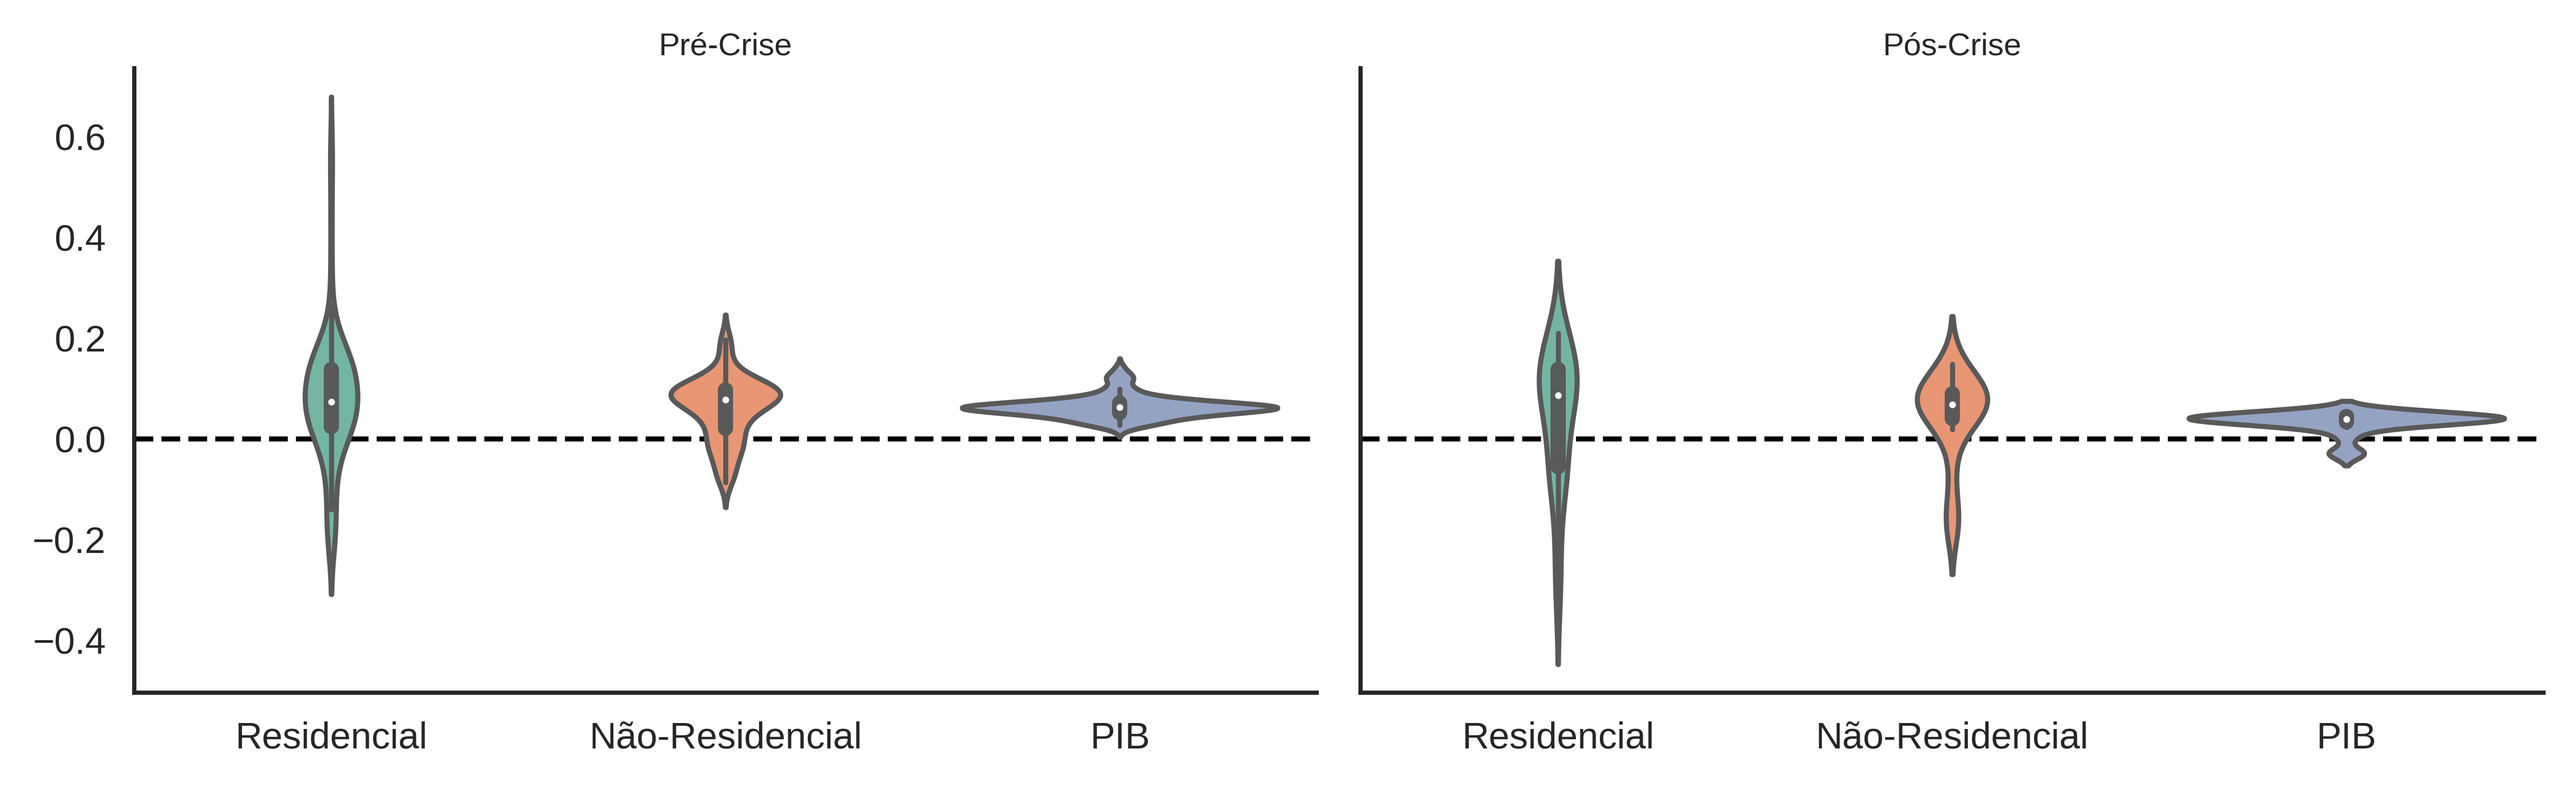
\includegraphics[width=\textwidth]{../../Dados/Fatos_Estilizados/figs/Volatilidade.png}
	\caption*{\textbf{Fonte:} U.S. Bureau of Economic Analisys, elaboração própria}
\end{figure}


\begin{figure}[H]
	\centering
	\caption{Participação dos gastos autônomos no PIB dos EUA (1979-2019)}
	\label{FigAutonomos}
	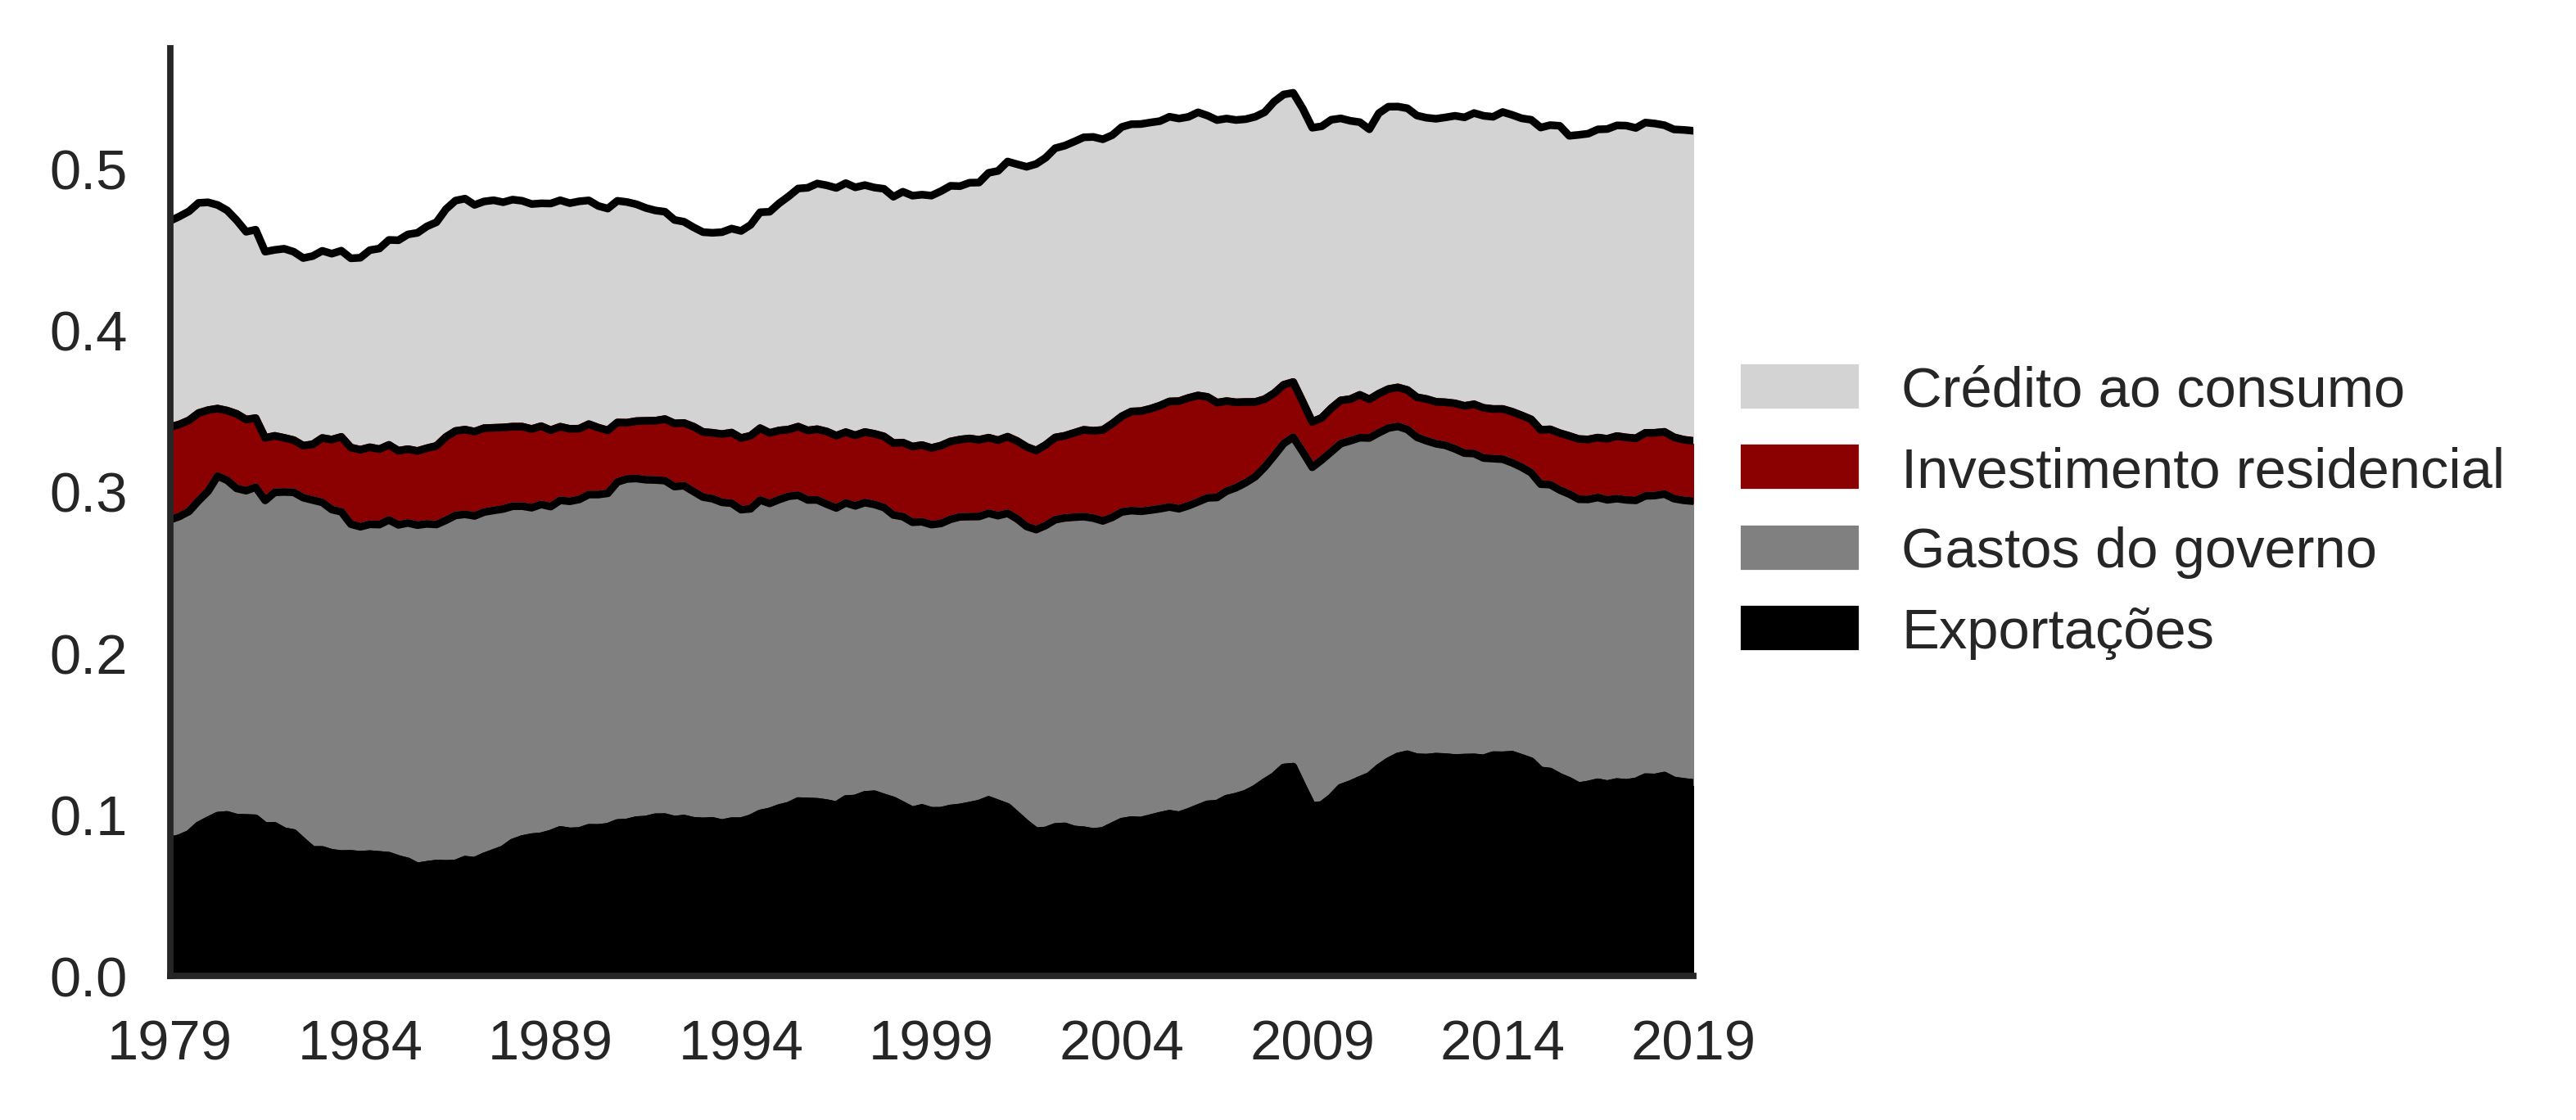
\includegraphics[width=\textwidth]{../../Dados/Fatos_Estilizados/figs/Gastos_autonomos.png}
	\caption*{\textbf{Fonte:} U.S. Bureau of Economic Analisys, elaboração própria}
\end{figure}

Neste ponto, cabe mencionar o ineditismo de \textcite{green_follow_1997} e \textcite{leamer_housing_2007} --- e revisitado em \textcite{leamer_housing_2015} e por \textcite{fiebiger_trend_2017} --- ao lançar luz sobre a importância do investimento residencial na determinação dos ciclos econômicos antes mesmo da Grande Recessão. 
Ao avaliar o caso norte-americano, \textcite{green_follow_1997} conclui que o
investimento residencial antecipa --- mais que o investimento das firmas --- o ciclo econômico, mas, ao mesmo tempo, reconhece que isso não implica o estabelecimento de uma relação causal. Na tentativa de compreender tais resultados, afirma:

\begin{citacao}
	
	[P]\textit{erhaps residential investiment, like stock prices and interest rates, is a good predictor of GDP because it is a series that reflects \textbf{foward looking behavior}. Presumably households will not increase their expenditures on housing unless they expect to prosper in the future. Building a house is a natural mechanism for doing this. Thus, the series can do a good job of predicting GDP without necessarily causing GDP}.
	\cite[p.~267, grifos adicionados]{green_follow_1997}
\end{citacao}
Apesar de dar atenção para um gasto não criador de capacidade, \textcite{green_follow_1997} restringe a importância do investimento residencial enquanto indicador de uma precedência temporal, ou seja, contribui para prever a trajetória da renda sem necessariamente causá-la.
\textcite{leamer_housing_2007}, por sua vez, avança em direção a relação de causalidade entre este gasto e o PIB. Grosso modo, afirma que a construção de novos imóveis implica maior consumo de bens duráveis e, portanto, trata-se de um ciclo decorrente do \textit{volume} e não do preço dos imóveis. 

Uma forma de visualizar a importância do investimento residencial para o ciclo econômico na economia estadunidense é por meio do gráfico \ref{FigIh_u} em que cada um dos painéis apresenta um ciclo iniciado no primeiro trimestre de crescimento positivo após a recessão e se estende até o fim da recessão seguinte\footnote{
	Raciocínio semelhante pode ser encontrado em \textcite{fiebiger_semi-autonomous_2018} em que, diferentemente do presente trabalho, não é incluído consumo financiado por crédito.}. 
No eixo vertical, observa-se a participação desse gasto no PIB, enquanto no eixo horizontal, o grau de utilização da capacidade como uma \textit{proxy} para o ciclo econômico. Exceto para o período 1991-2001, a recuperação (aumento da utilização da capacidade) é caracterizada por uma taxa de crescimento do investimento residencial maior que o crescimento da economia, resultando em maior participação desse gasto no PIB. Considerando que as firmas seguem o princípio do ajuste do estoque de capital, ampliam a taxa de acumulação de modo a ajustar o grau de utilização para o grau normal. O aumento da taxa de crescimento do investimento das firmas e de outros gastos reduz a participação do investimento residencial no PIB. A maturação do investimento das firmas, por sua vez, redunda em menor utilização da capacidade produtiva\footnote{
	Complementarmente, os trabalhos de \textcite{fiebiger_semi-autonomous_2018} e \textcite{fiebiger_trend_2017} também reportam o investimento residencial como determinante do comportamento cíclico e adicionam o consumo financiado por crédito a essa dinâmica. Além disso, apresentam uma similaridade com \textcite{dejuan_hidden_2017} e \textcite{teixeira_crescimento_2015} para os quais a instabilidade econômica está associada à instabilidade (ao menos de alguns) gastos autônomos e não do investimento das firmas, que segue o princípio do ajuste do estoque de capital.}. 
Com o deflagrar da crise, o grau de utilização cai e o ciclo se encerra no fim da recessão e se reinicia --- no painel seguinte --- com a economia sendo puxada pelo investimento residencial.
Em resumo, tais gráficos denotam uma especifidade do ciclo econômico norte-americano que pode ser resumida nos seguintes termos: ``\textit{[f]irst homes, then cars, and last business equipment}'' \cite[p.~8]{leamer_housing_2007}.




\begin{figure}[H]
	\centering
	\caption{Relação entre taxa de investimento residencial e grau de utilização por recessão}
	\label{FigIh_u}
	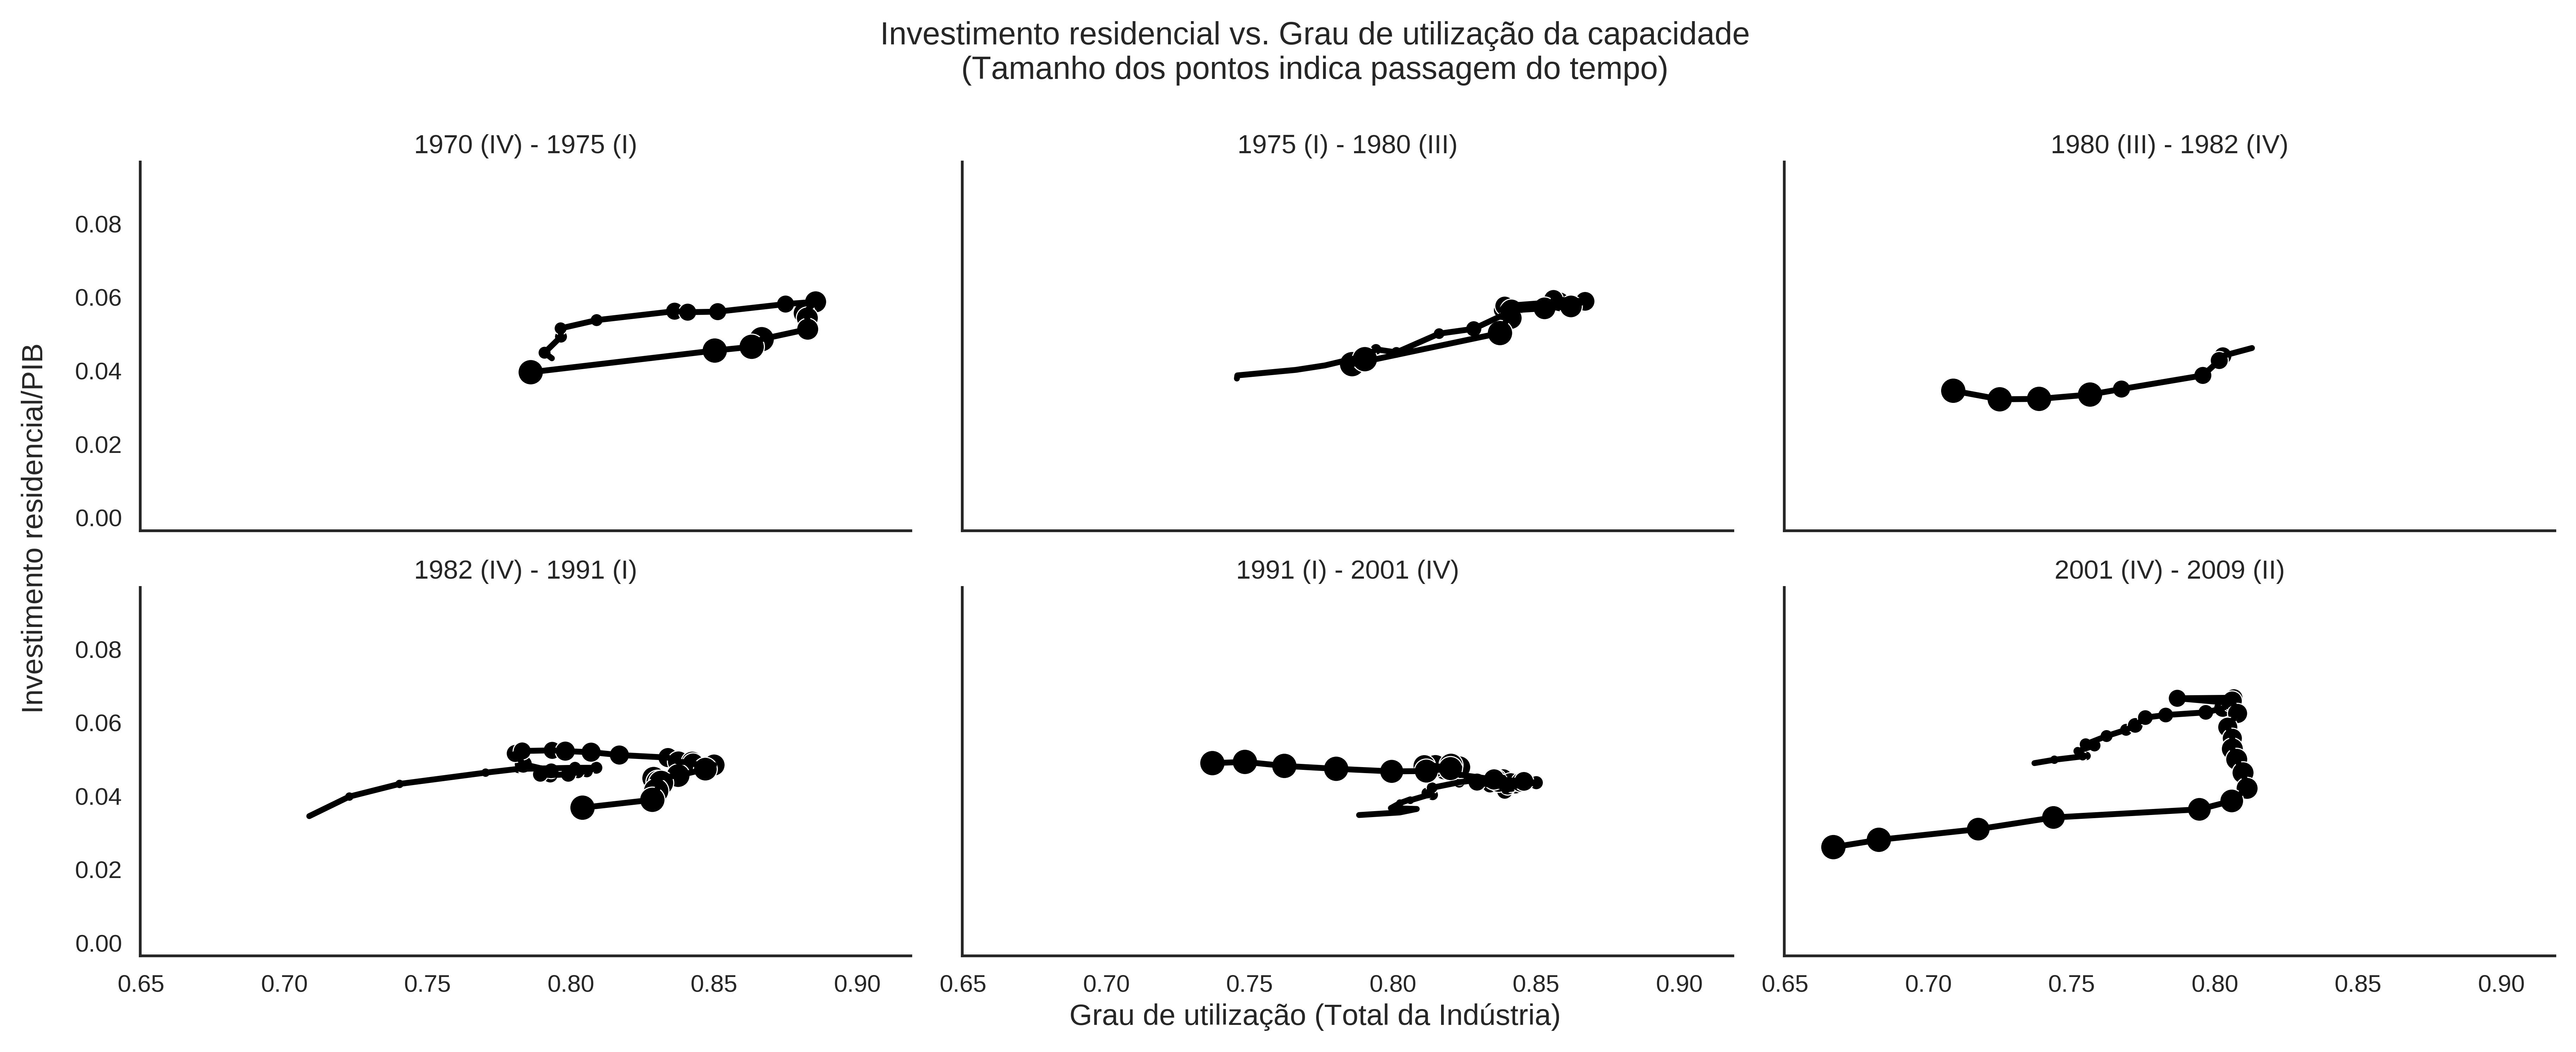
\includegraphics[width=\textwidth]{../../Dados/Fatos_Estilizados/figs/Ciclo_Ih_u.png}
	\caption*{\textbf{Fonte:} Elaboração própria}
\end{figure}

%%%%%%%%%%%%%%%%%%%%%%% GRÁFICO RELÓGIO DURÁVEIS %%%%%%%%%%%%%%%%%%

%Como mencionado anteriormente, além de liderar o ciclo econômico, o investimento residencial também está relacionado com o consumo de bens duráveis.
%O gráfico \ref{FigInvesto_Duraveis} ilustra tal associação em que é feita a mesma periodização das crises dos painéis anteriores com a diferença de que o eixo horizontal apresenta a participação do consumo de bens duráveis na renda. 
%Diferentemente do gráfico anterior, este não apresenta um comportamento cíclico tão demarcado ao longo do período que antecedeu a Grande Recessão. Apesar disso, é possível visualizar que a economia desacelera na medida que estes gastos decrescem (conjuntamente) enquanto o crescimento conjunto destes gastos na recuperação não é tão evidente em todos os ciclos (destaque para o ciclo de 1975 a 1980).

%\begin{figure}[H]
%	\centering
%	\caption{Relação entre taxa de investimento residencial e grau de utilização por recessão}
%	\label{FigInvesto_Duraveis}
%	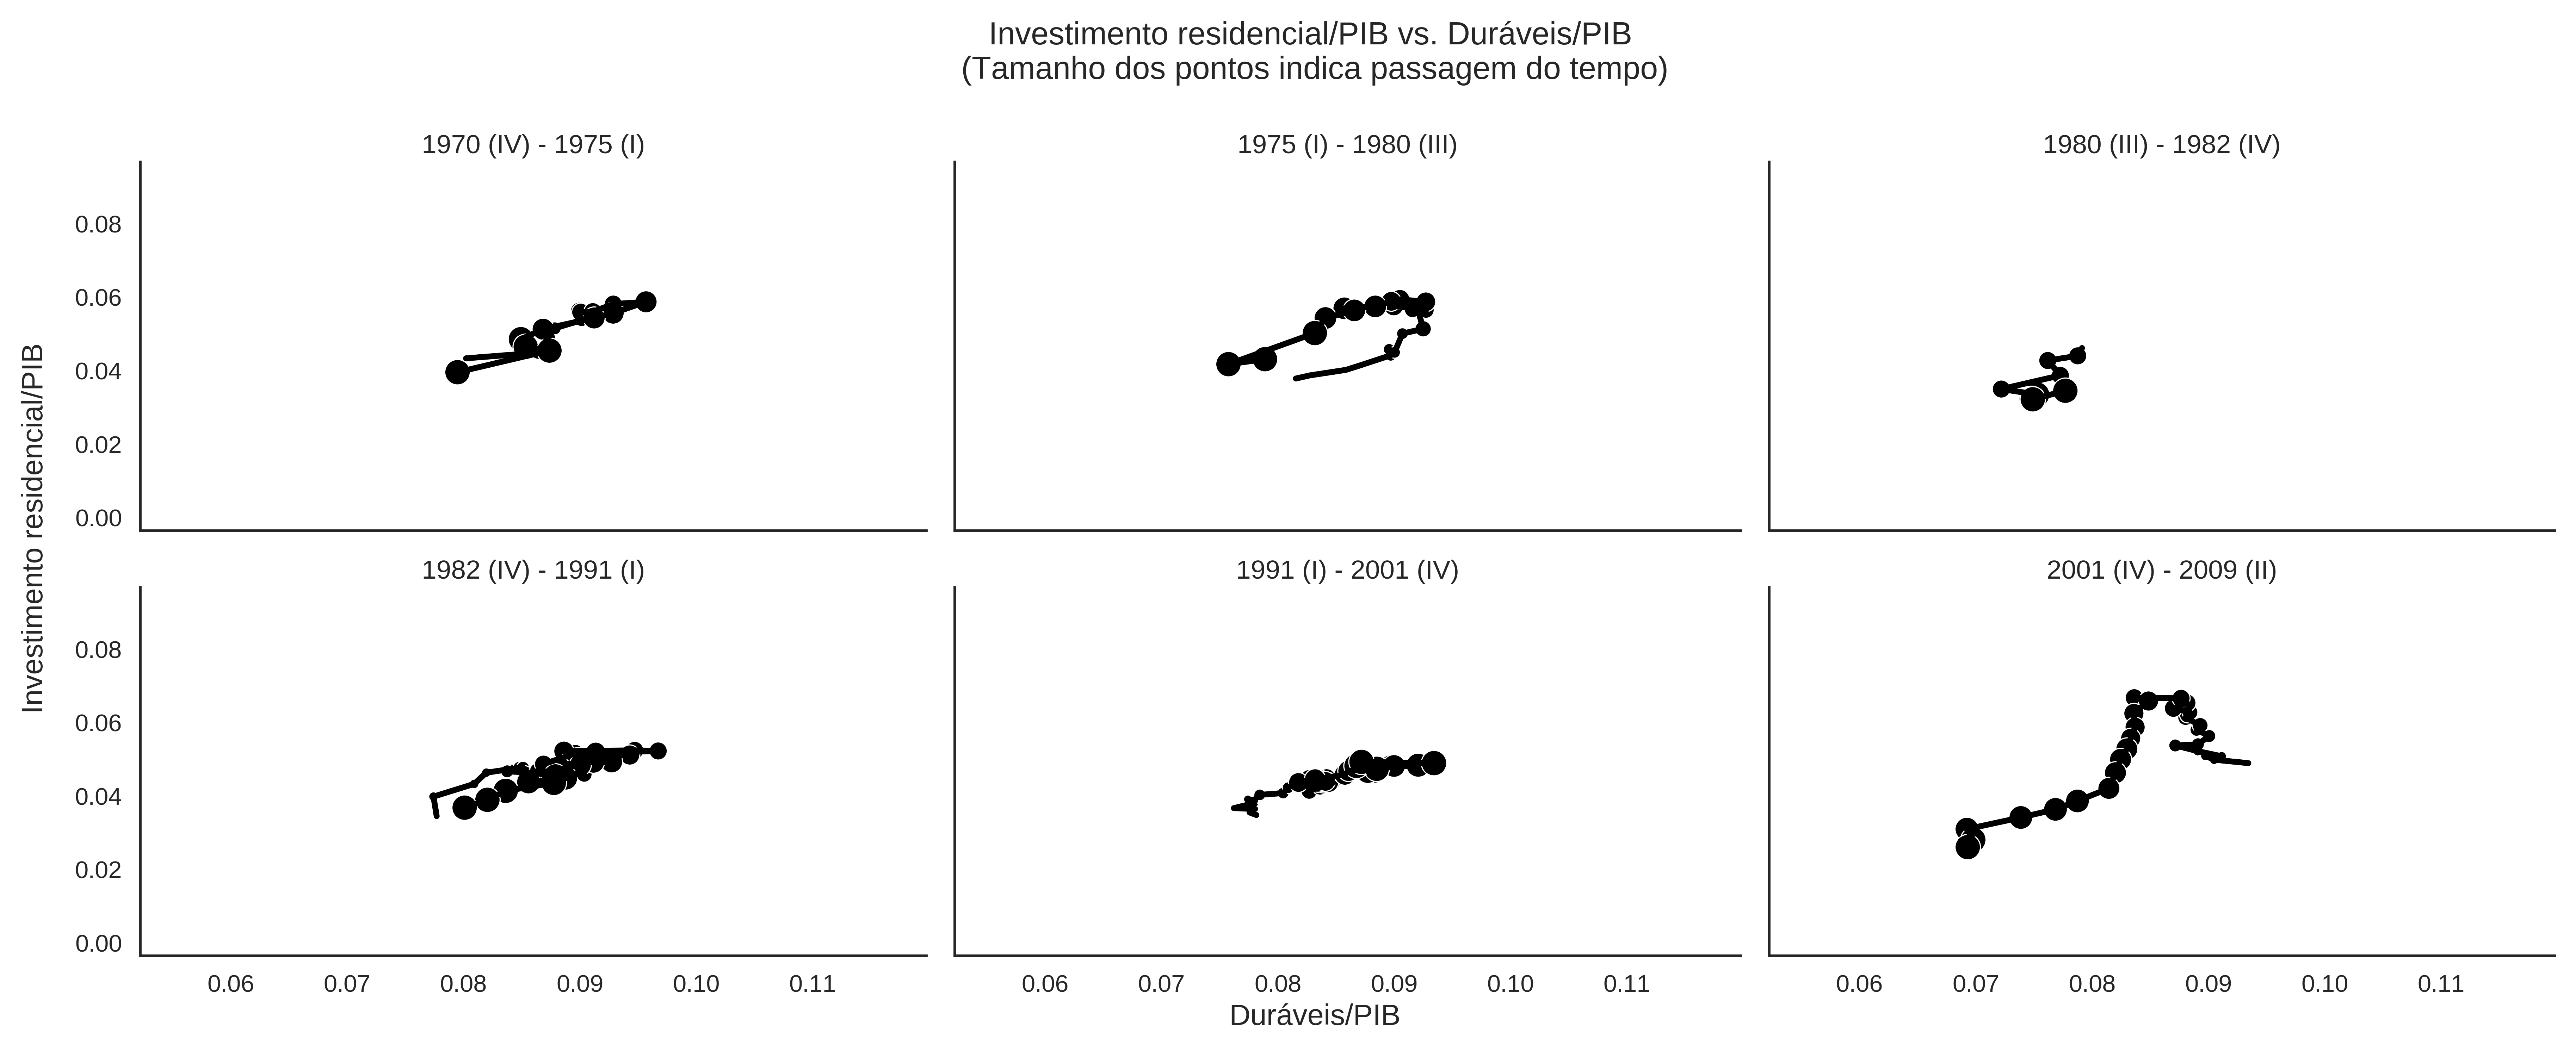
\includegraphics[width=\textwidth]{../../Dados/Fatos_Estilizados/figs/Ciclo_Ih_Duraveis.png}
%	\caption*{\textbf{Fonte:} Elaboração própria}
%\end{figure}

%Desse modo, conclui-se que o investimento residencial ajuda a compreender os ciclos econômicos americanos.
%Esta dinâmica pode ser visualizada também nos gráficos \ref{FigCriseNorm} e \ref{FigRecuperacaoNorm} em que são apresentadas as taxas de crescimento do produto, consumo financiado por crédito, investimento residencial e não-residencial (normalizadas para manter a comparabilidade)\footnote{
%	Nestes gráficos, as taxas de crescimento são normalizadas para facilitar a comparabilidade uma vez que é mantida uma mesma escala uma vez que o investimento residencial apresenta uma taxa de crescimento mais ampla em relação às demais. 
%	Dito isso, normalizou-se a taxa de crescimento por seu respectivo desvio-padrão.
%} nos trimestres que antecedem e sucedem as recessões/recuperações. 
%Destaca-se a redução da taxa de crescimento do investimento residencial nos trimestres que antecedem as recessões enquanto passa a ter taxas positivas antes das recuperações, liderando-as.
%Em outras palavras, observa-se que o investimento residencial possui uma taxa de crescimento (a taxas crescentes) positiva nos trimestres que antecedem a recuperação enquanto o investimento das firmas só apresenta tal comportamento adiante. Portanto, esse gráfico ilustra tanto a capacidade do investimento residencial liderar o ciclo quanto a indução do investimento criador de capacidade produtiva.
%
%
%\begin{figure}[H]
%	\centering
%	\caption{Taxas de crescimento 4 trimestres antes e depois do início da  \textbf{recessão} (normalizadas para manter a comparabilidade)}
%	\label{FigCriseNorm}
%	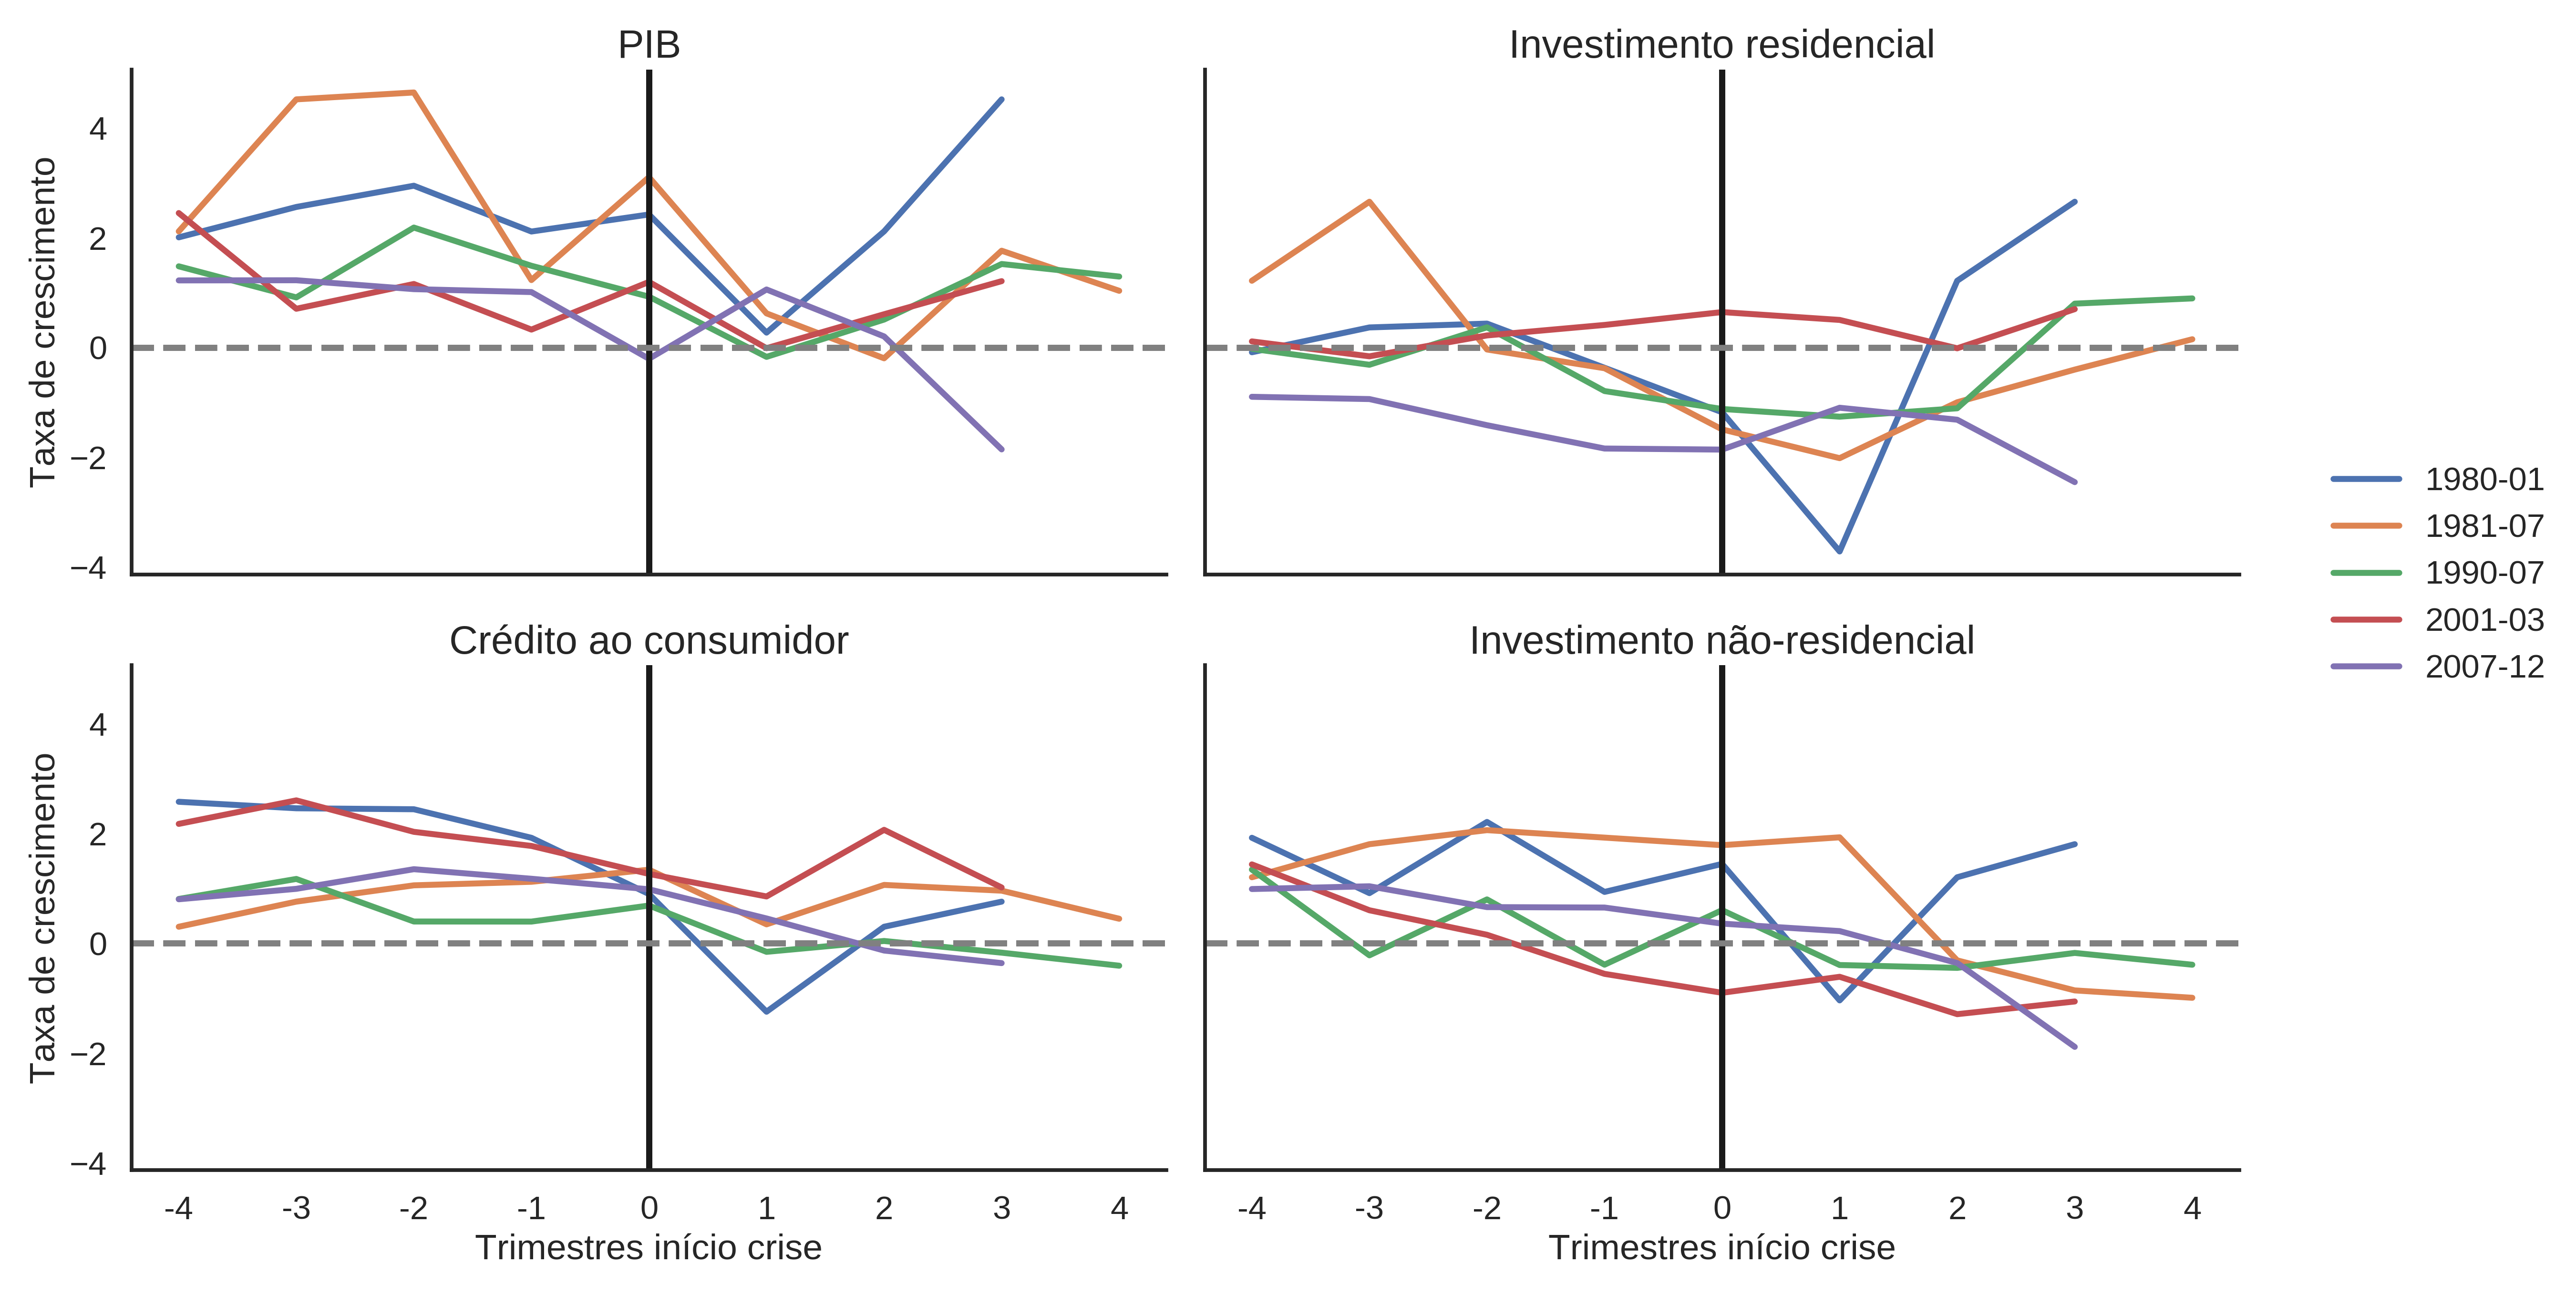
\includegraphics[width=\textwidth]{../../Dados/Fatos_Estilizados/figs/Centrado_Inicio_Norm.png}
%	\caption*{\textbf{Fonte:} Elaboração própria}
%\end{figure}
%
%\begin{figure}[H]
%	\centering
%	\caption{Taxas de crescimento 4 trimestres antes e depois do início da  \textbf{recuperação} (normalizadas para manter a comparabilidade)}
%	\label{FigRecuperacaoNorm}
%	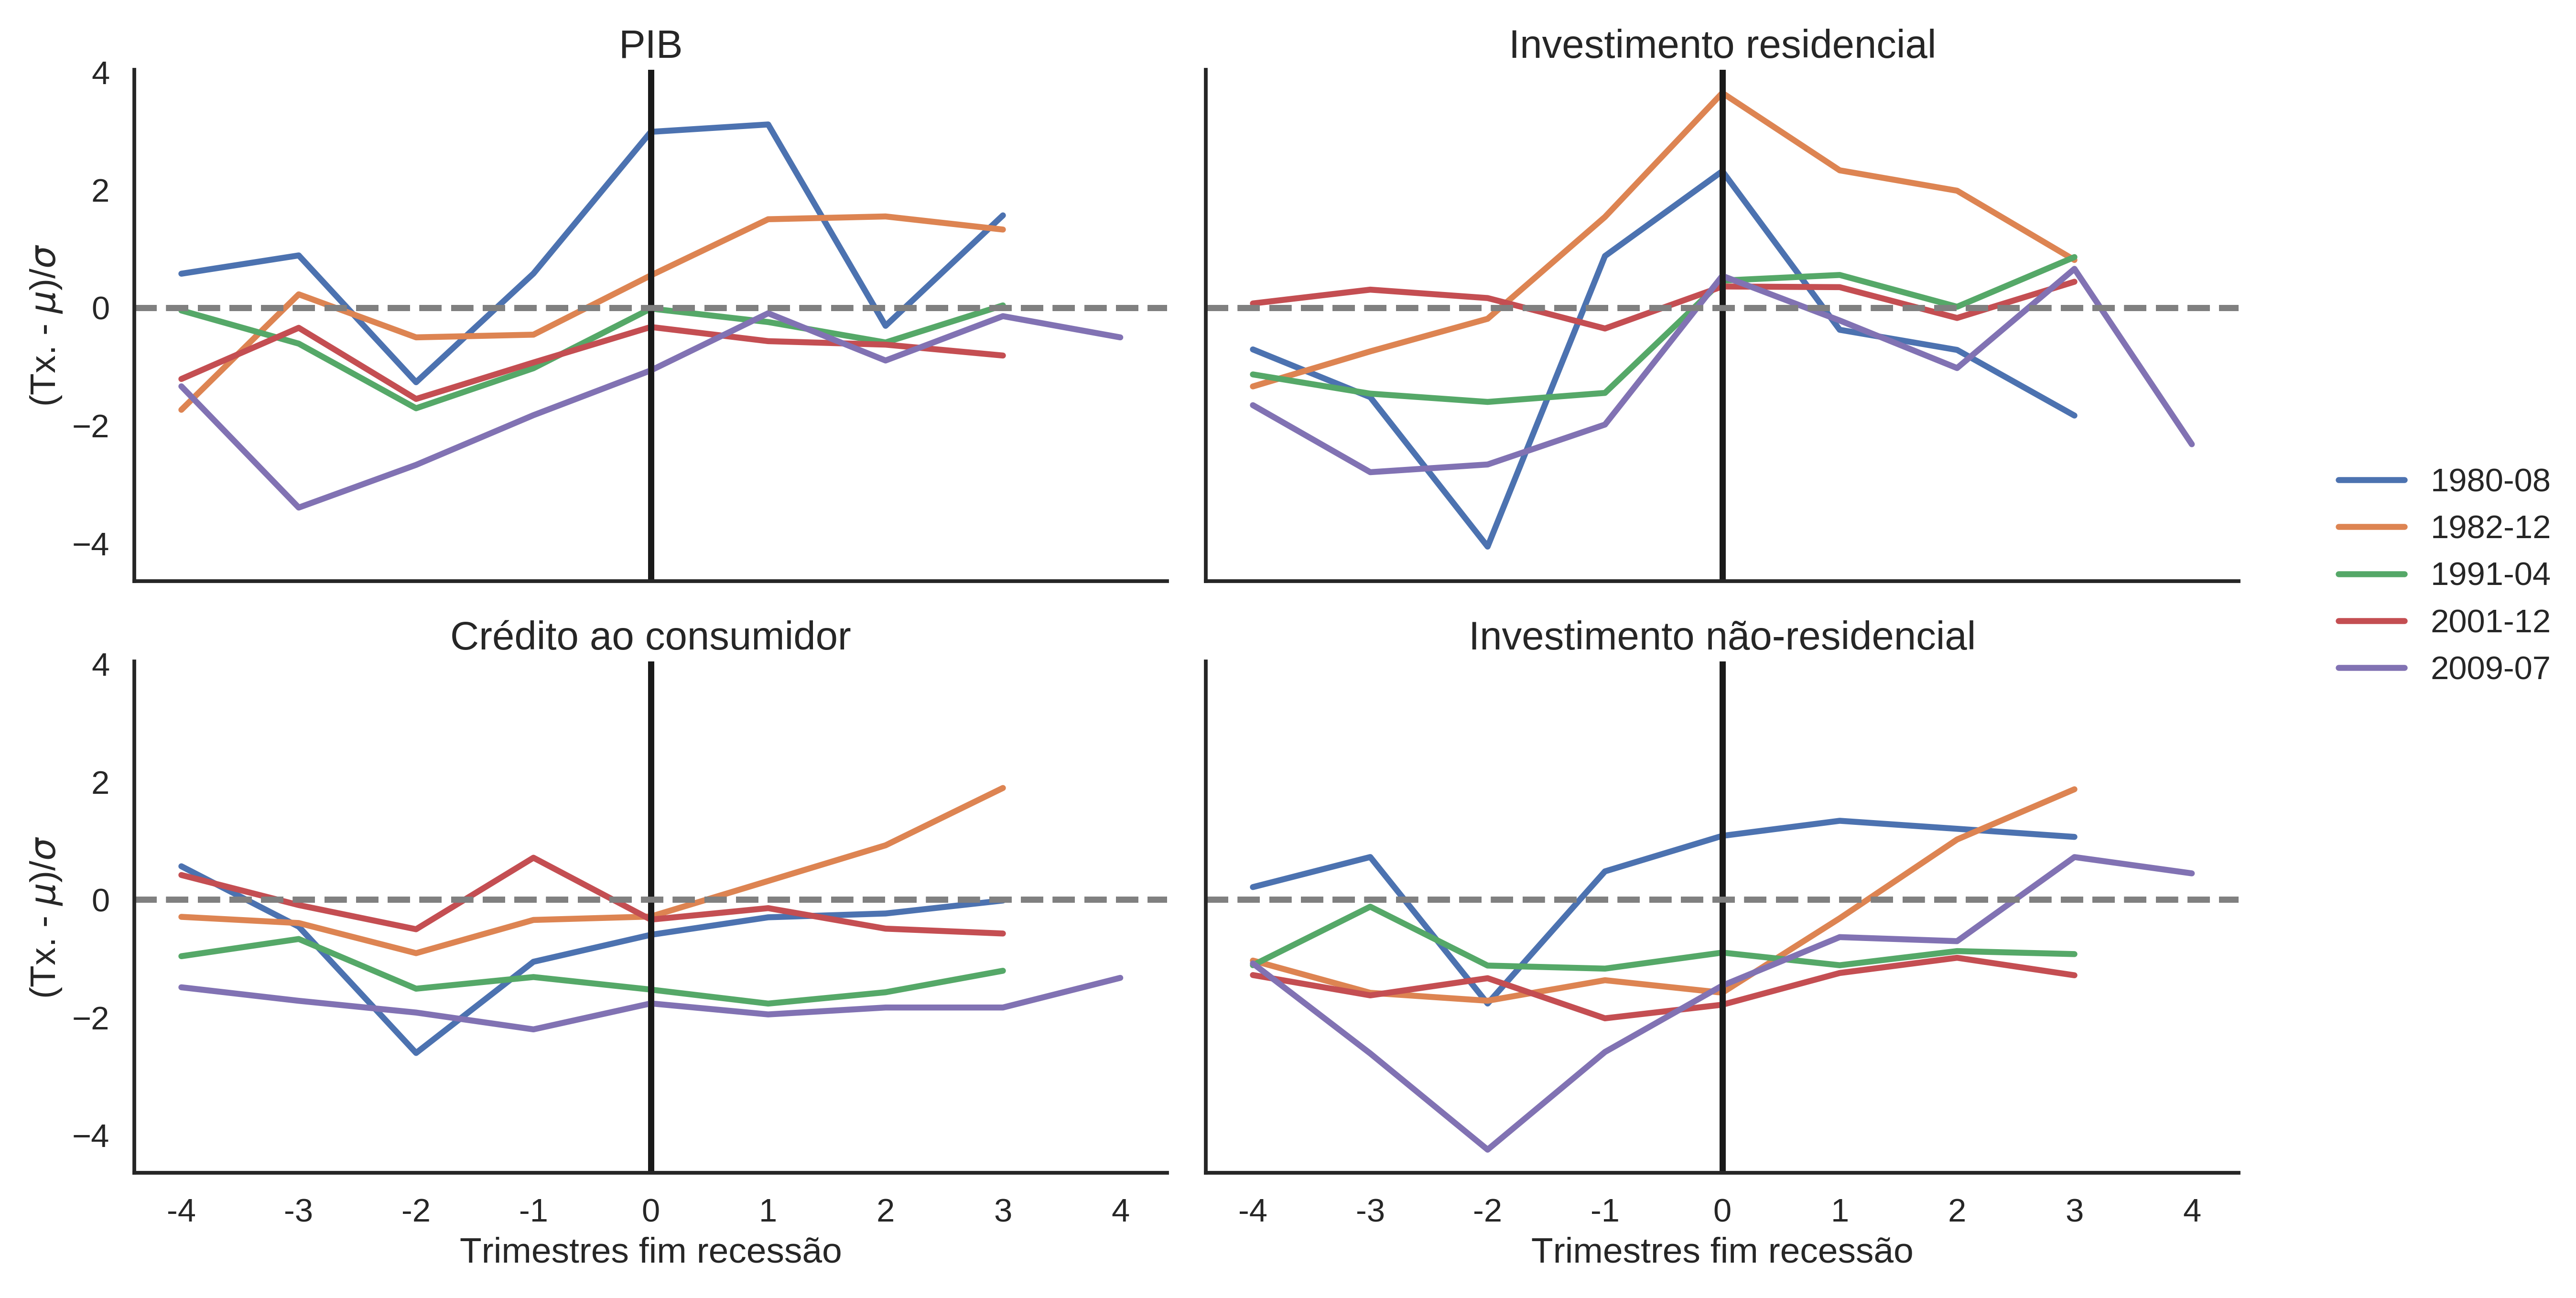
\includegraphics[width=\textwidth]{../../Dados/Fatos_Estilizados/figs/Centrado_Fim_Norm.png}
%	\caption*{\textbf{Fonte:} Elaboração própria}
%\end{figure}
%
%%TODO Melhorar resolução do gráfico e linhas


Da discussão anterior, conclui-se que a caracterização do ciclo econômico como liderado pelo investimento residencial é bastante extensa uma vez que apresenta esta configuração ao menos desde o pós-guerra.
Apresentada a importância do investimento residencial, resta pontuar alguns fatos estilizados da economia norte-americana que servirão de inspiração para a simulação no capítulo \ref{CapModelo}. 
%No entanto, ocorreram mudanças significantes --- que não anulam a relevância do investimento residencial --- na economia norte-americana no pós-década de 80 que precisam ser analisadas em maior detalhe.
%Um primeiro elemento é a estagnação salarial e os respectivos efeitos sobre o endividamento das famílias na calda inferior da distribuição \cites{barba_rising_2009}{teixeira_uma_2011}. 
%Este endividamento, no entanto, não foi destinado a uma ampliação desproporcional do consumo, mas sim para a preservação do consumo habitual das famílias
%\cites{wolf_rising_2010}{cynamon_inequality_2013}.
Um deles é a evolução dos ativos por percentis da riqueza (gráfico \ref{FigDistAtivos}) em que se destaca o aumento da participação relativa dos imóveis
nos 50\% mais pobres se comparado com 1979 até meados dos anos 90 ---  comportamento este espelhado pelos 1\% mais ricos. 
%Em outras palavras, os imóveis passaram a compor uma parcela cada vez maior do portfólio de ativos deste estrato enquanto os ativos financeiros apresentaram uma tendência de queda persistente.
Enquanto a participação dos imóveis dentre os mais pobres foi crescente e oscilante ao longo do período, o mesmo não pode ser dito sobre os bens duráveis.
Além disso, este gráfico também sugere que a demanda por imóveis por motivos especulativos foi iniciada pelo estrato dos 1\% mais ricos e acompanhada pelo subsequente aumento na demanda por imóveis --- não necessariamente especulativa --- dos 50\% mais pobres associada à expansão do crédito e à desregulamentação financeira.


%\begin{figure}[H]
%	\centering
%	\caption{Distribuição pessoal da renda (percentis selecionados, jan/1980 = 100)}
%	\label{FigDistPessoal}
%	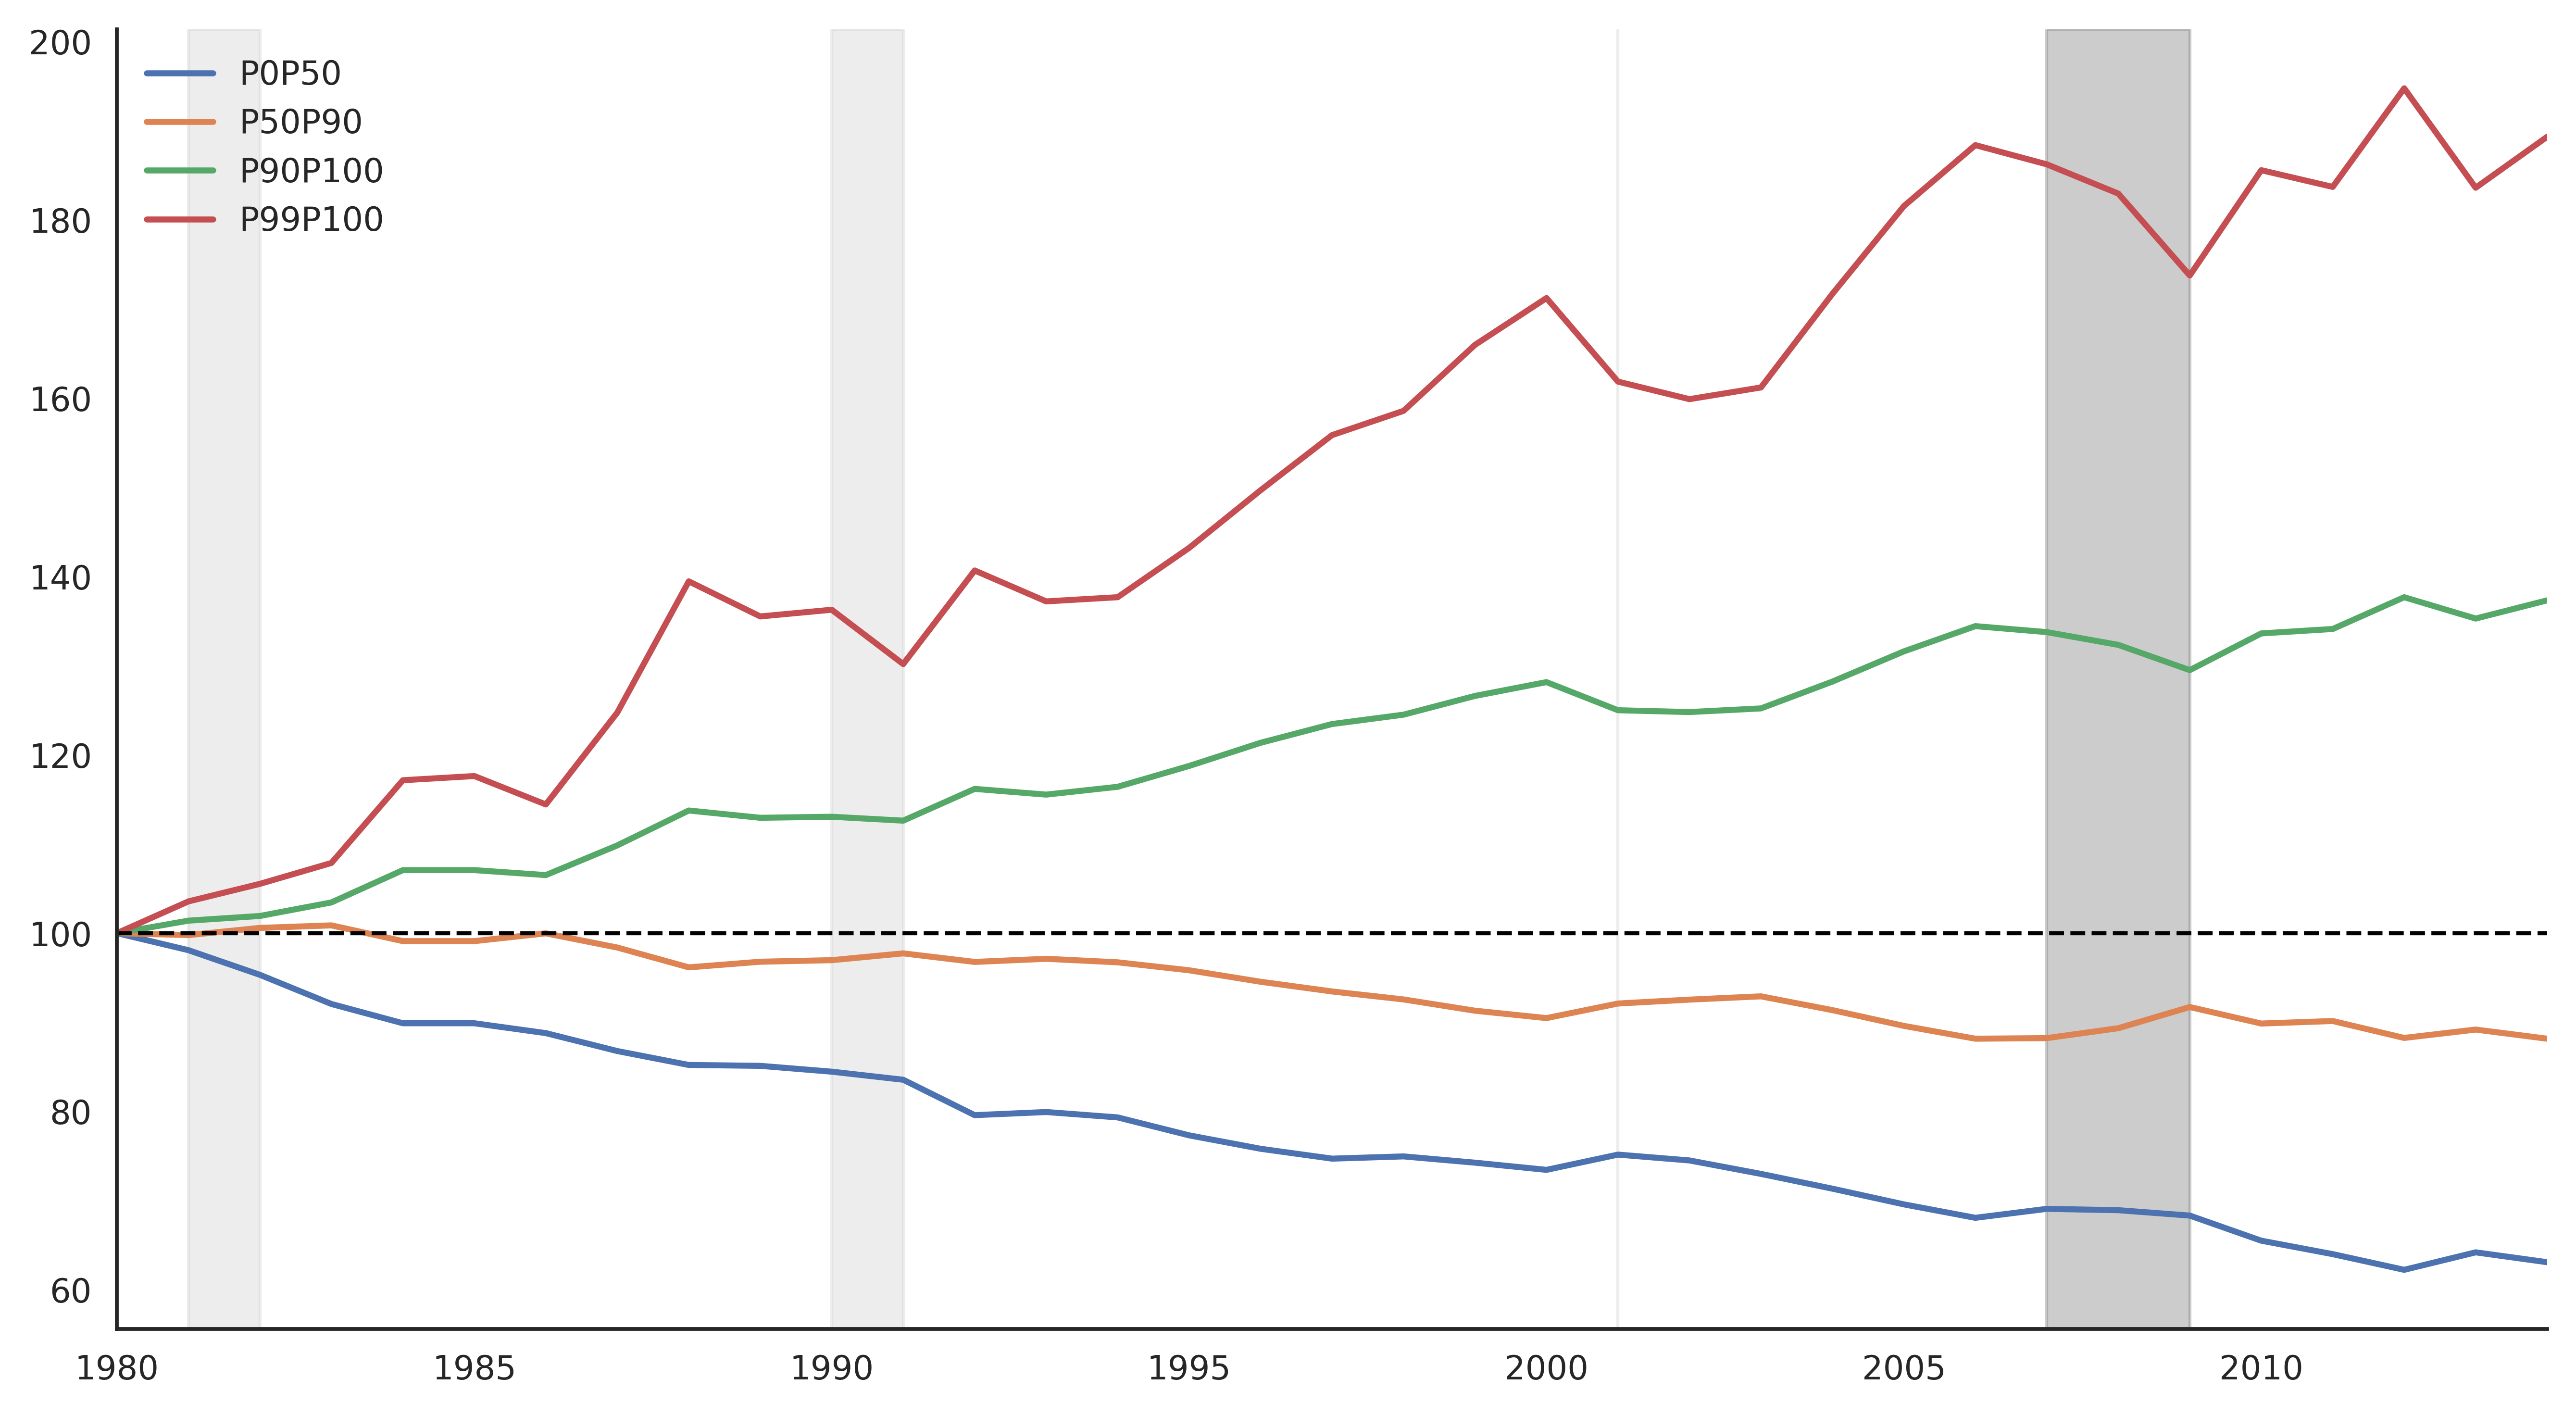
\includegraphics[width=\textwidth]{../../Dados/Fatos_Estilizados/figs/Dist_Pessoal.png}
%	\caption*{\textbf{Fonte:} World Inequality Database (WID), elaboração própria}
%\end{figure}



\begin{figure}[H]
	\centering
	\caption{Evolução de ativos por percentil de riqueza (1989/07=1)}
	\label{FigDistAtivos}
	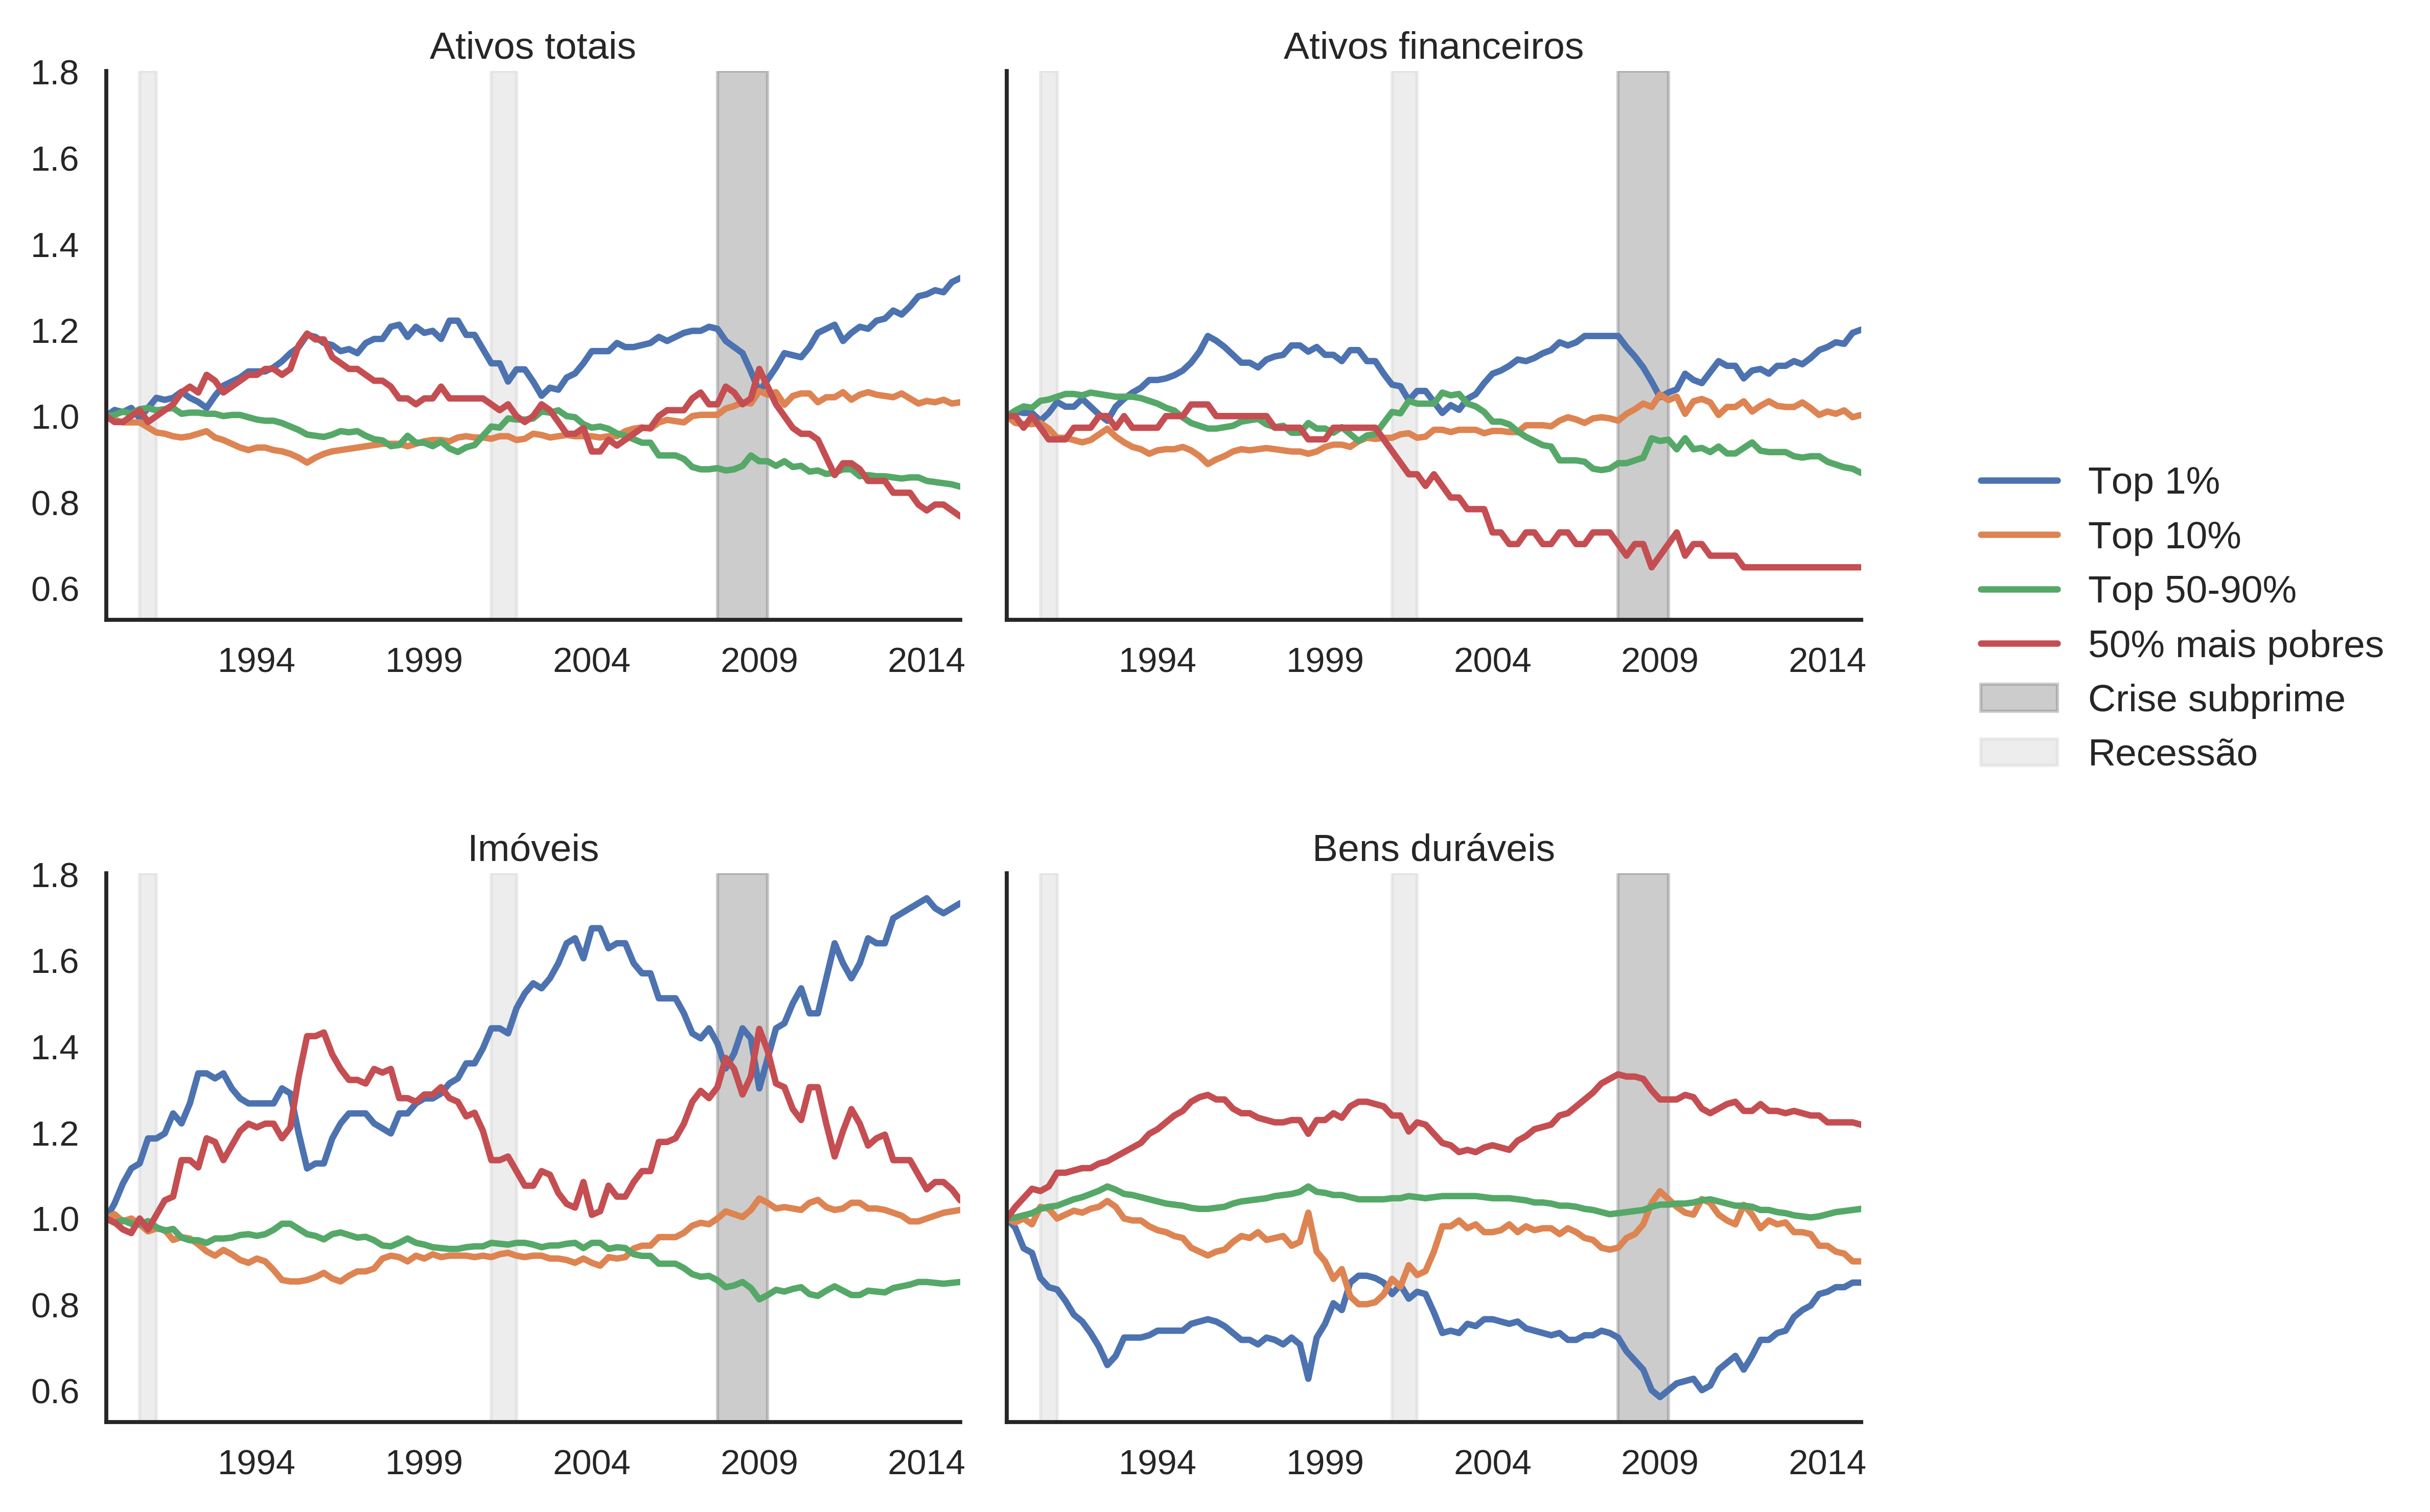
\includegraphics[width=\textwidth]{../../Dados/Fatos_Estilizados/figs/Distribuicao_Ativos.png}
	\caption*{\textbf{Fonte:} \textcite{us_census_bureau_characteristics_2017}, Elaboração própria}
\end{figure}

Os passivos (gráfico \ref{FigDistPassivos}), por sua vez, apresentam uma dinâmica semelhante entre si, ou seja, a participação nos empréstimos e nas hipotecas  é bastante similar ao longo do período analisado.
Argumenta-se aqui que tal resultado decorre da permissividade institucional americana.
De acordo com \textcite{teixeira_uma_2011}, os imóveis são uma das formas de riqueza mais comuns entre as famílias norte-americanas, servindo de colateral para tomada de crédito. A forma de ``realizar'' o ganho de capital com a bolha imobiliária que ocorreu no período, sem precisar liquidar os imóveis, era justamente ampliando o endividamento à medida que o colateral (\textit{i.e.} imóveis) aumentava de valor \cite{teixeira_crescimento_2015}. 


\begin{figure}[H]
	\centering
	\caption{Evolução de passivos por percentil de riqueza (1989/07=1)}
	\label{FigDistPassivos}
	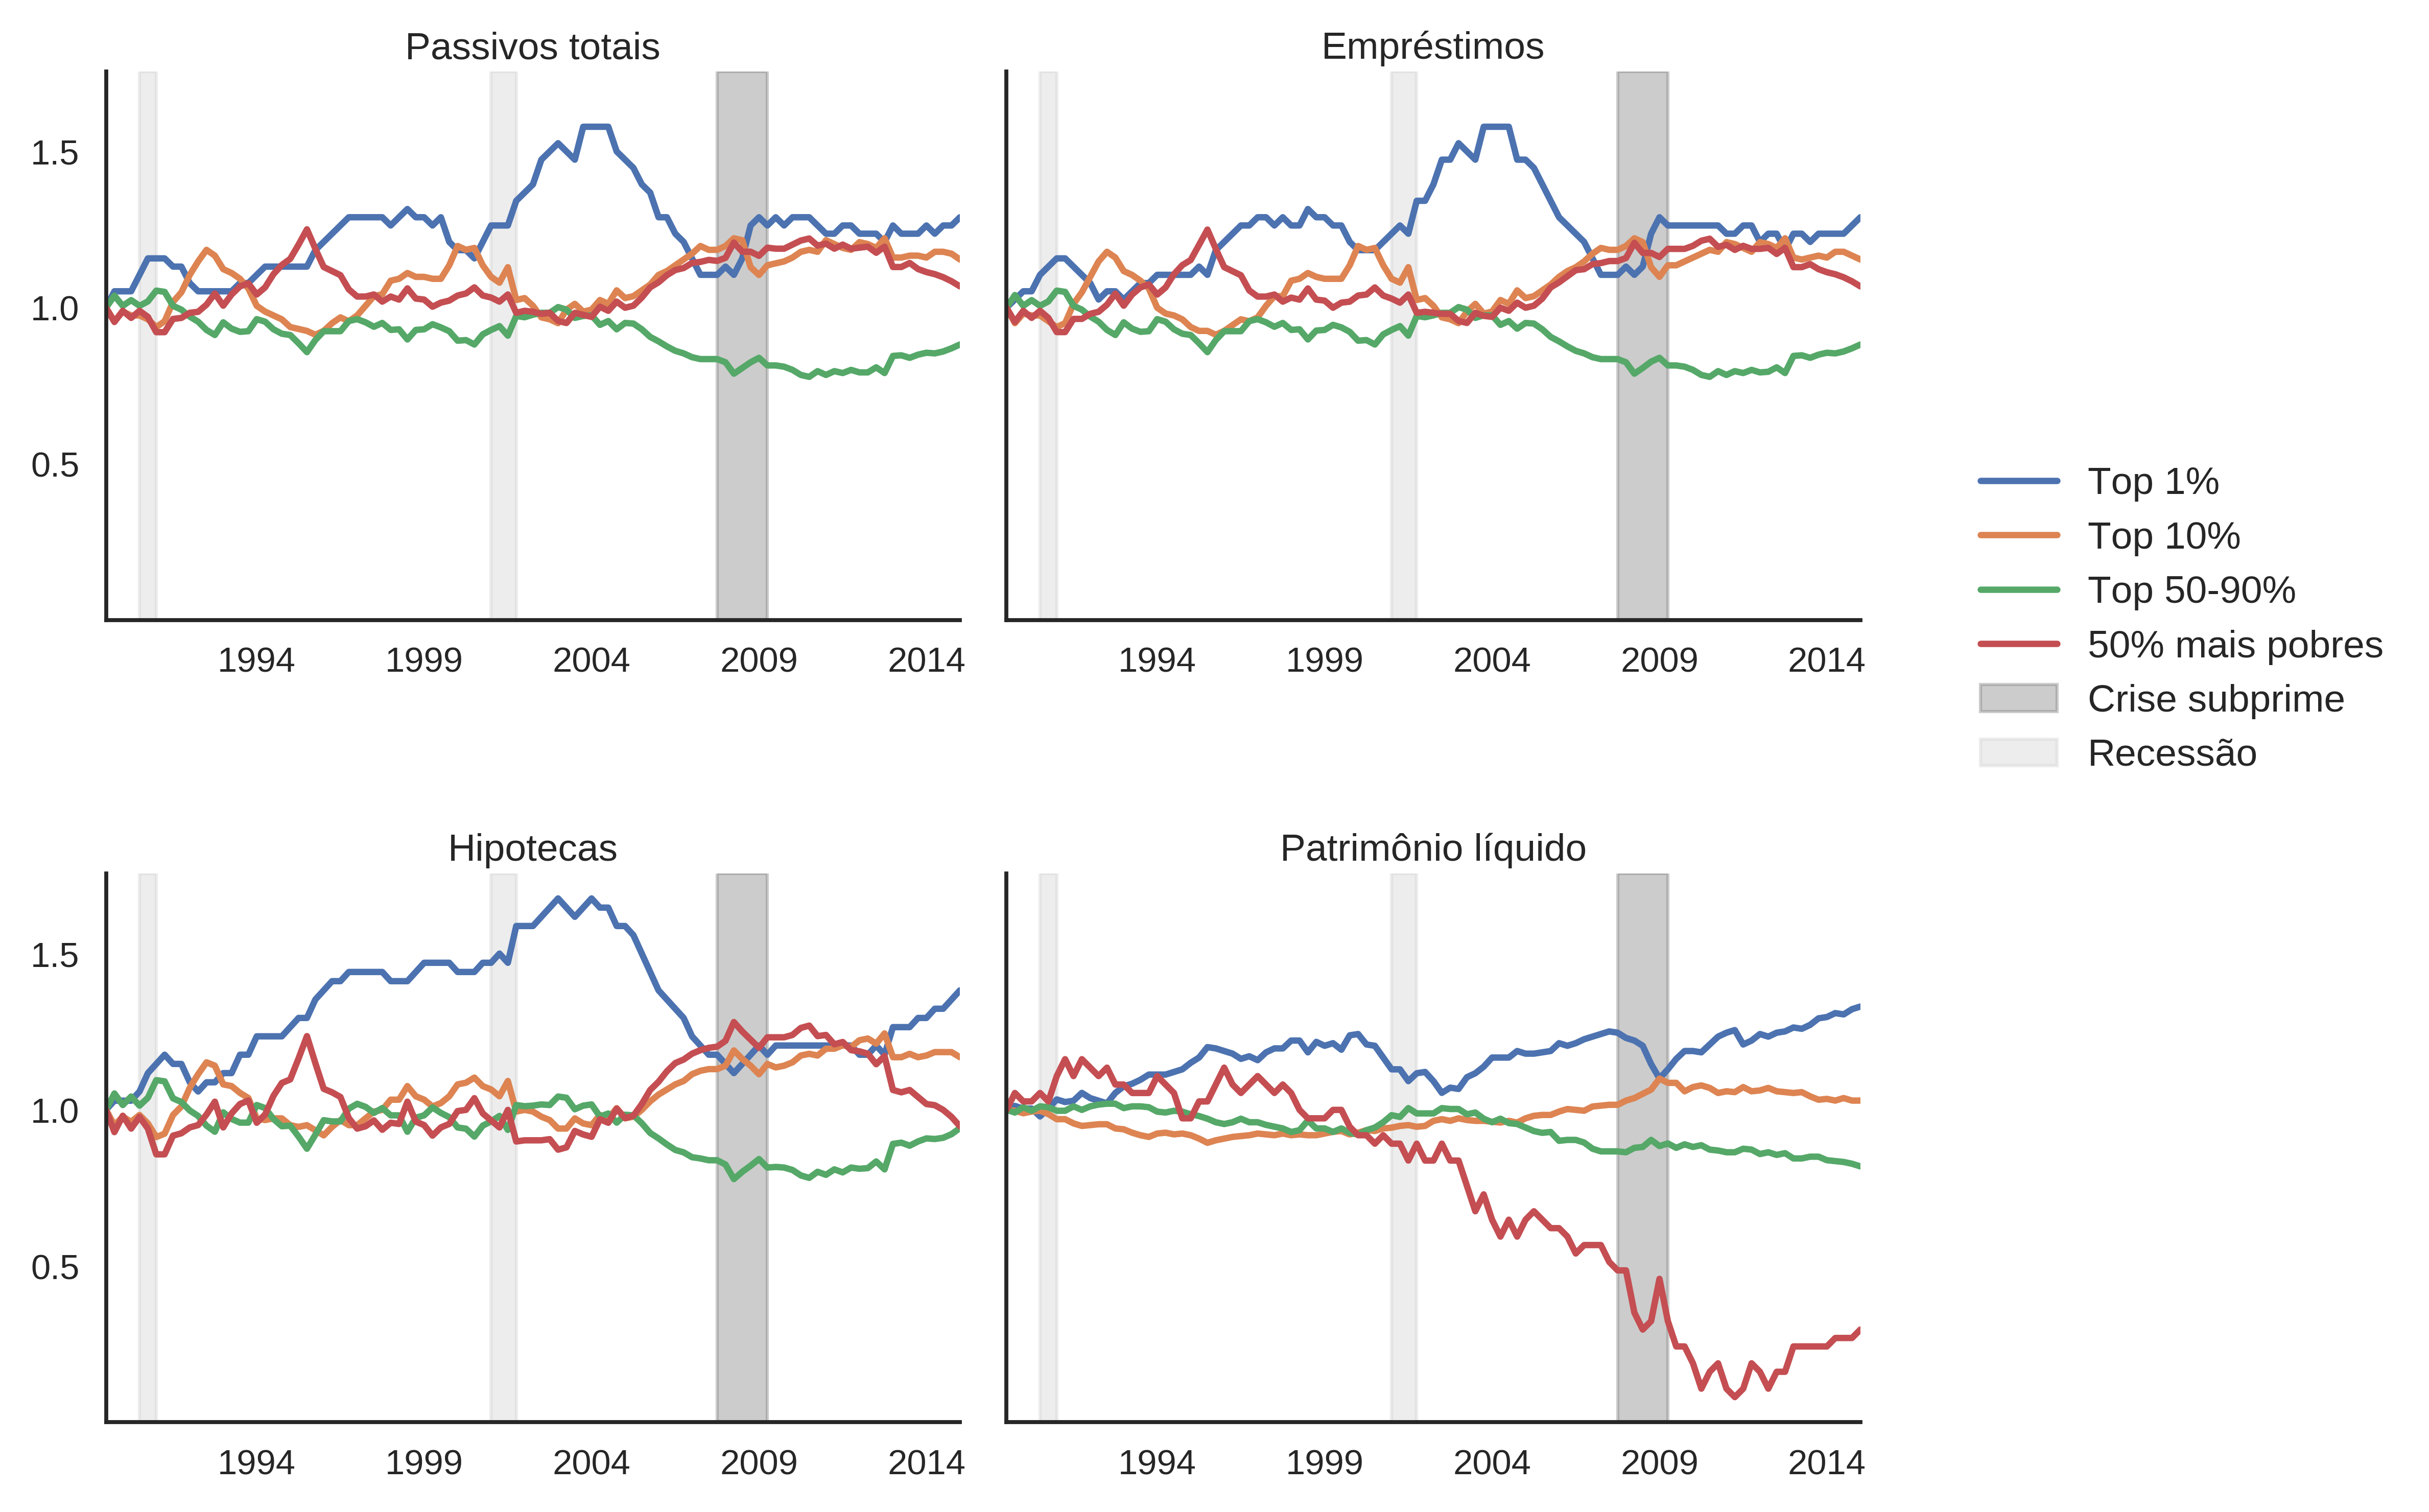
\includegraphics[width=\textwidth]{../../Dados/Fatos_Estilizados/figs/Distribuicao_Passivos.png}
	\caption*{\textbf{Fonte:} \textcite{us_census_bureau_characteristics_2017}, Elaboração própria}
\end{figure}


Como consequência, observa-se uma dinâmica gêmea (ver gráfico \ref{FigDividaPreco}) entre endividamento das famílias e preço dos imóveis que, por sua vez, permitia a ampliação do consumo --- sobretudo das famílias mais pobres --- mesmo com a estagnação salarial do período.
Tal especificidade institucional teve algumas implicações sobre a dinâmica macroeconômica que precisam ser melhor analisadas.
A primeira delas é o descolamento entre ativos e passivos no decorrer da crise financeira de 2008.
Esta separação decorre tanto do esgotamento da bolha dos imóveis (pós-2005) que fez com que os tais ativos desvalorizassem quanto da insensibilidade dos compromissos financeiros das famílias (\textit{i.e.} dívida) a queda do preço dos imóveis.
Em outras palavras, os imóveis (ativo) tem valor de mercado enquanto a dívida (passivo) tem um valor contratual sendo assim, o patrimônio líquido das famílias cai com o instaurar da crise.
A segunda implicação --- resultante da conjugação dos movimentos anteriores --- é a redução acentuada do patrimônio líquido das famílias mais pobres em termos absolutos e relativos (painel inferior direito do gráfico \ref{FigDistPassivos}).
%Em resumo, a estagnação dos salários somada às inovações financeiras que permitiram ampliação do consumo por meio de ampliação no colateral das famílias associado a elevação do preços dos imóveis resultaram em uma substituição dos salários por dívida \cite{barba_rising_2009}.


\begin{figure}[H]
	\centering
	\caption{Dinâmica do endividamento das famílias e do preço dos imóveis (jan/2000=100)}
	\label{FigDividaPreco}
	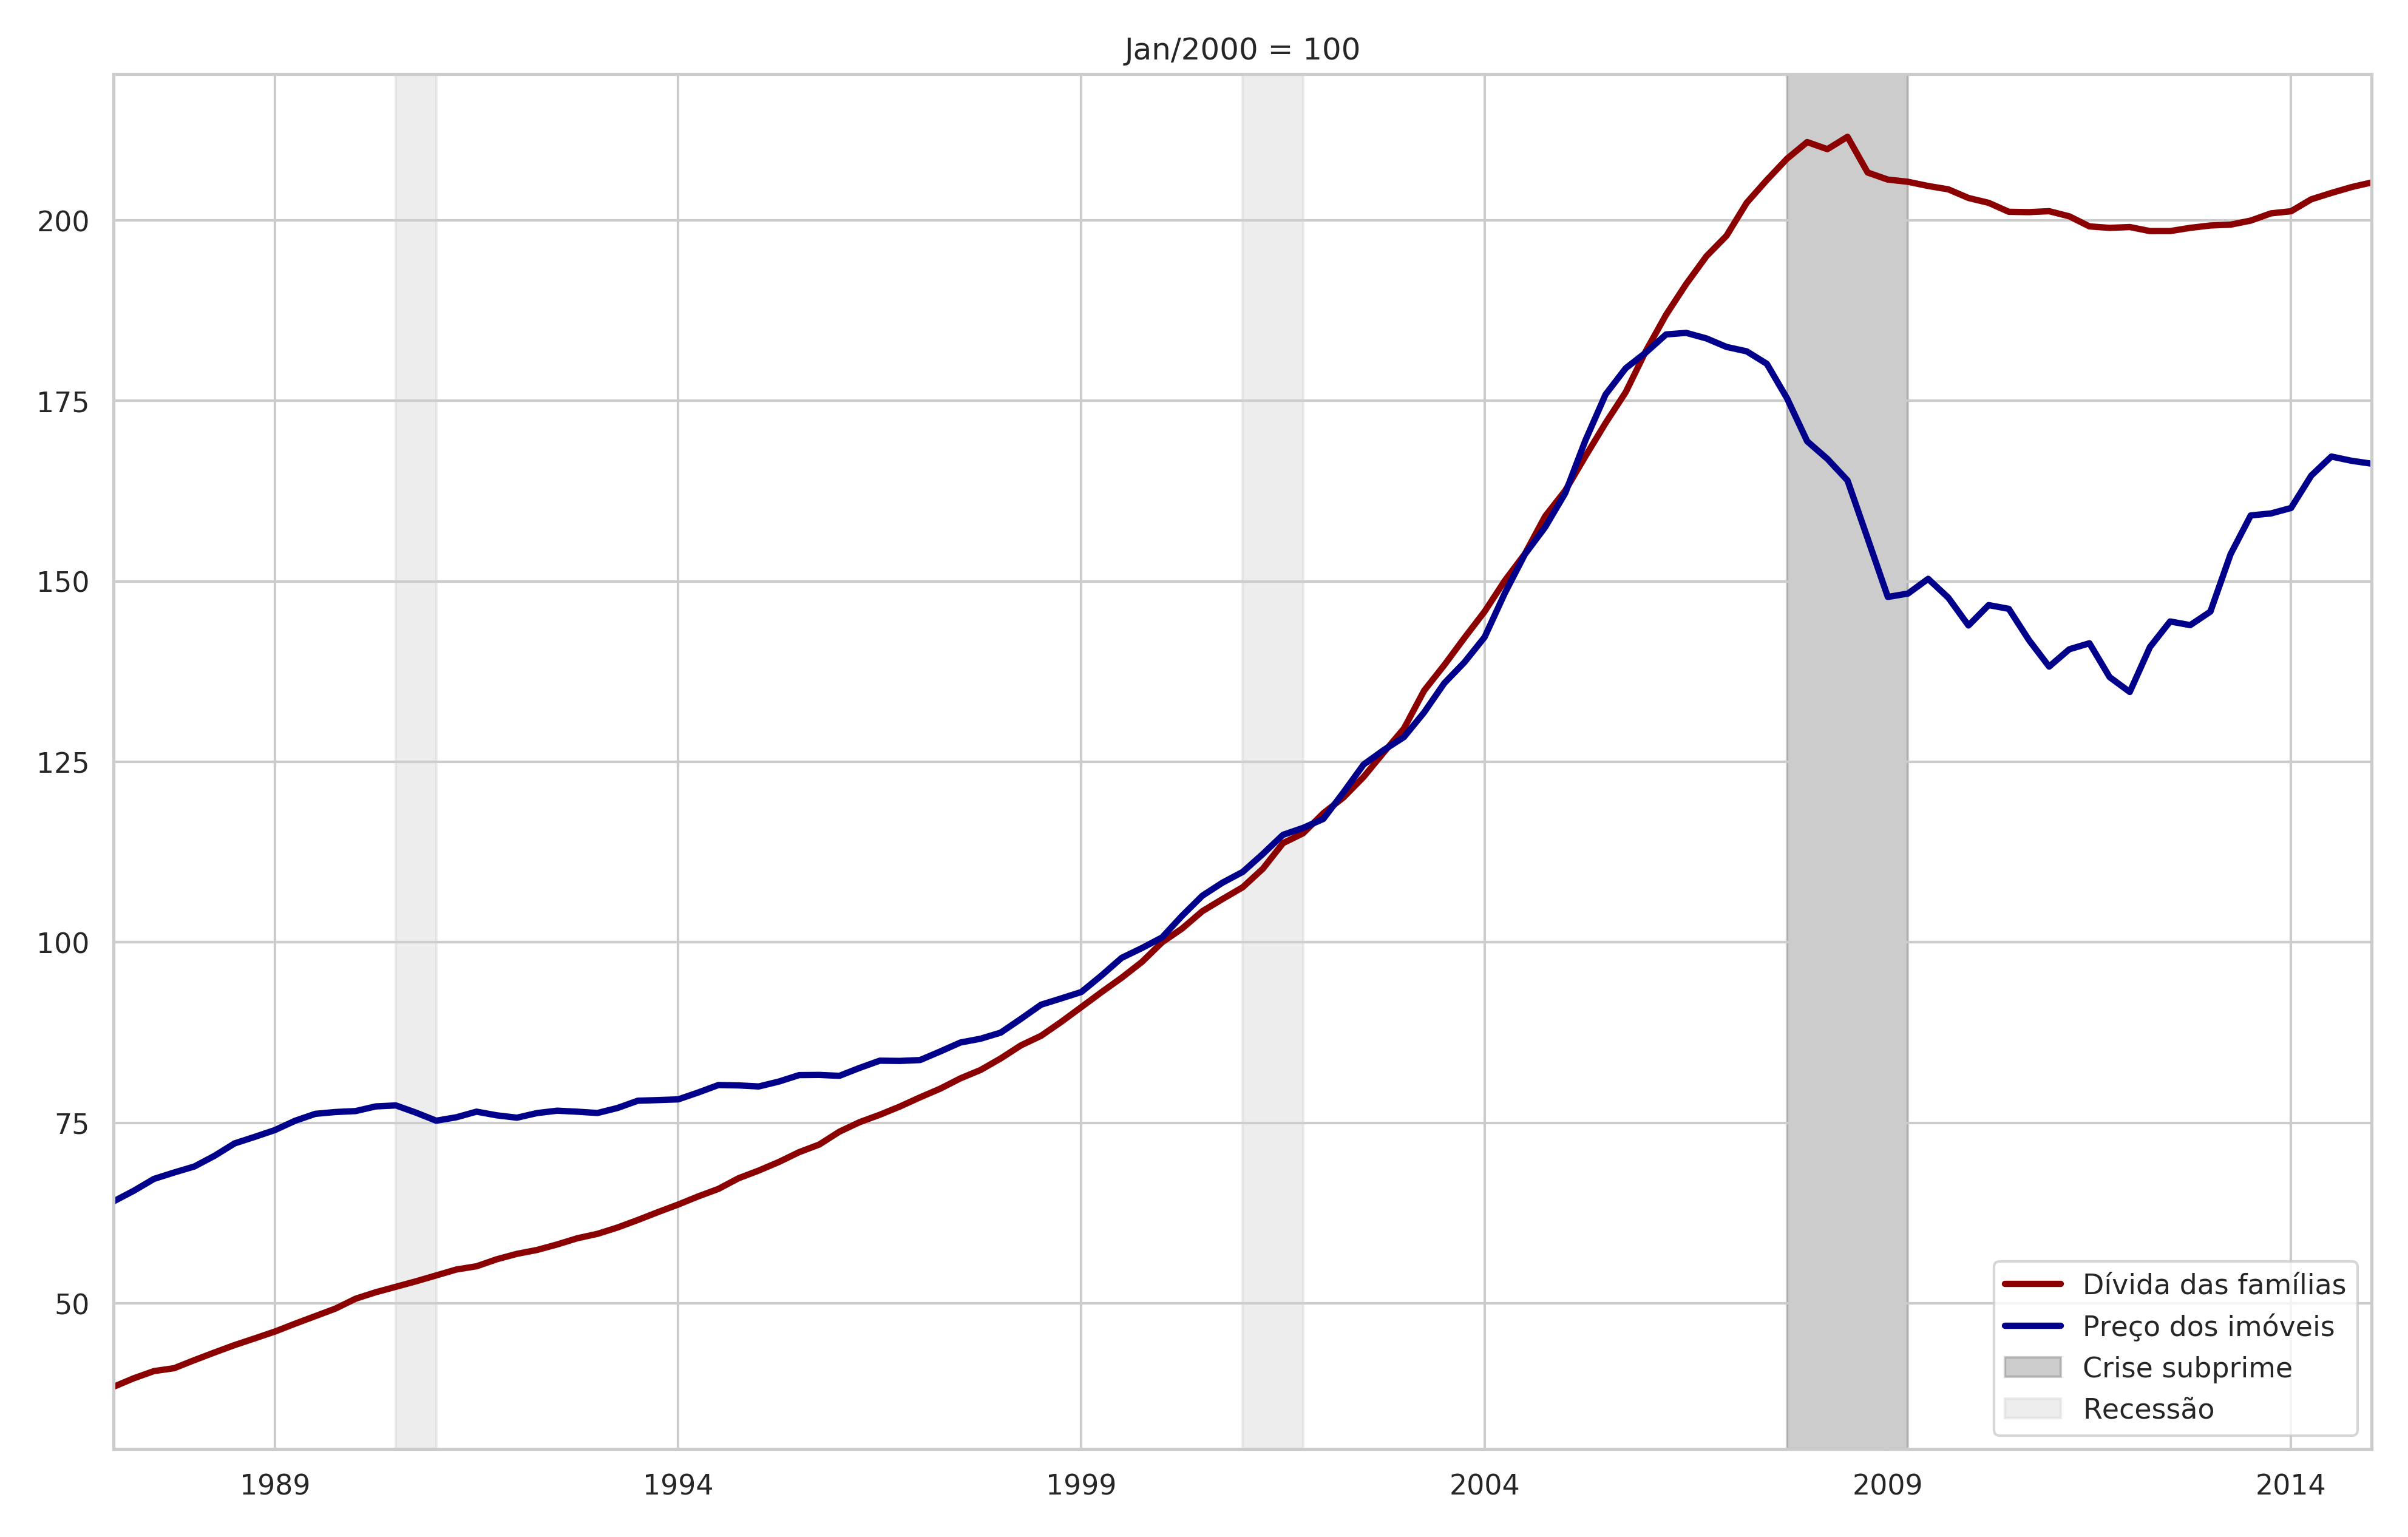
\includegraphics[width=\textwidth]{../../Dados/Fatos_Estilizados/figs/Divida_PrecoImoveis.png}
	\caption*{\textbf{Fonte:} U.S. Bureau of Economic Analisys, elaboração própria}
\end{figure}

%\begin{figure}[H]
%	\centering
%	\caption{Comprometimento da renda das famílias com o pagamento de juros (jan/1980 = 100)}
%	\label{FigServDiv}
%	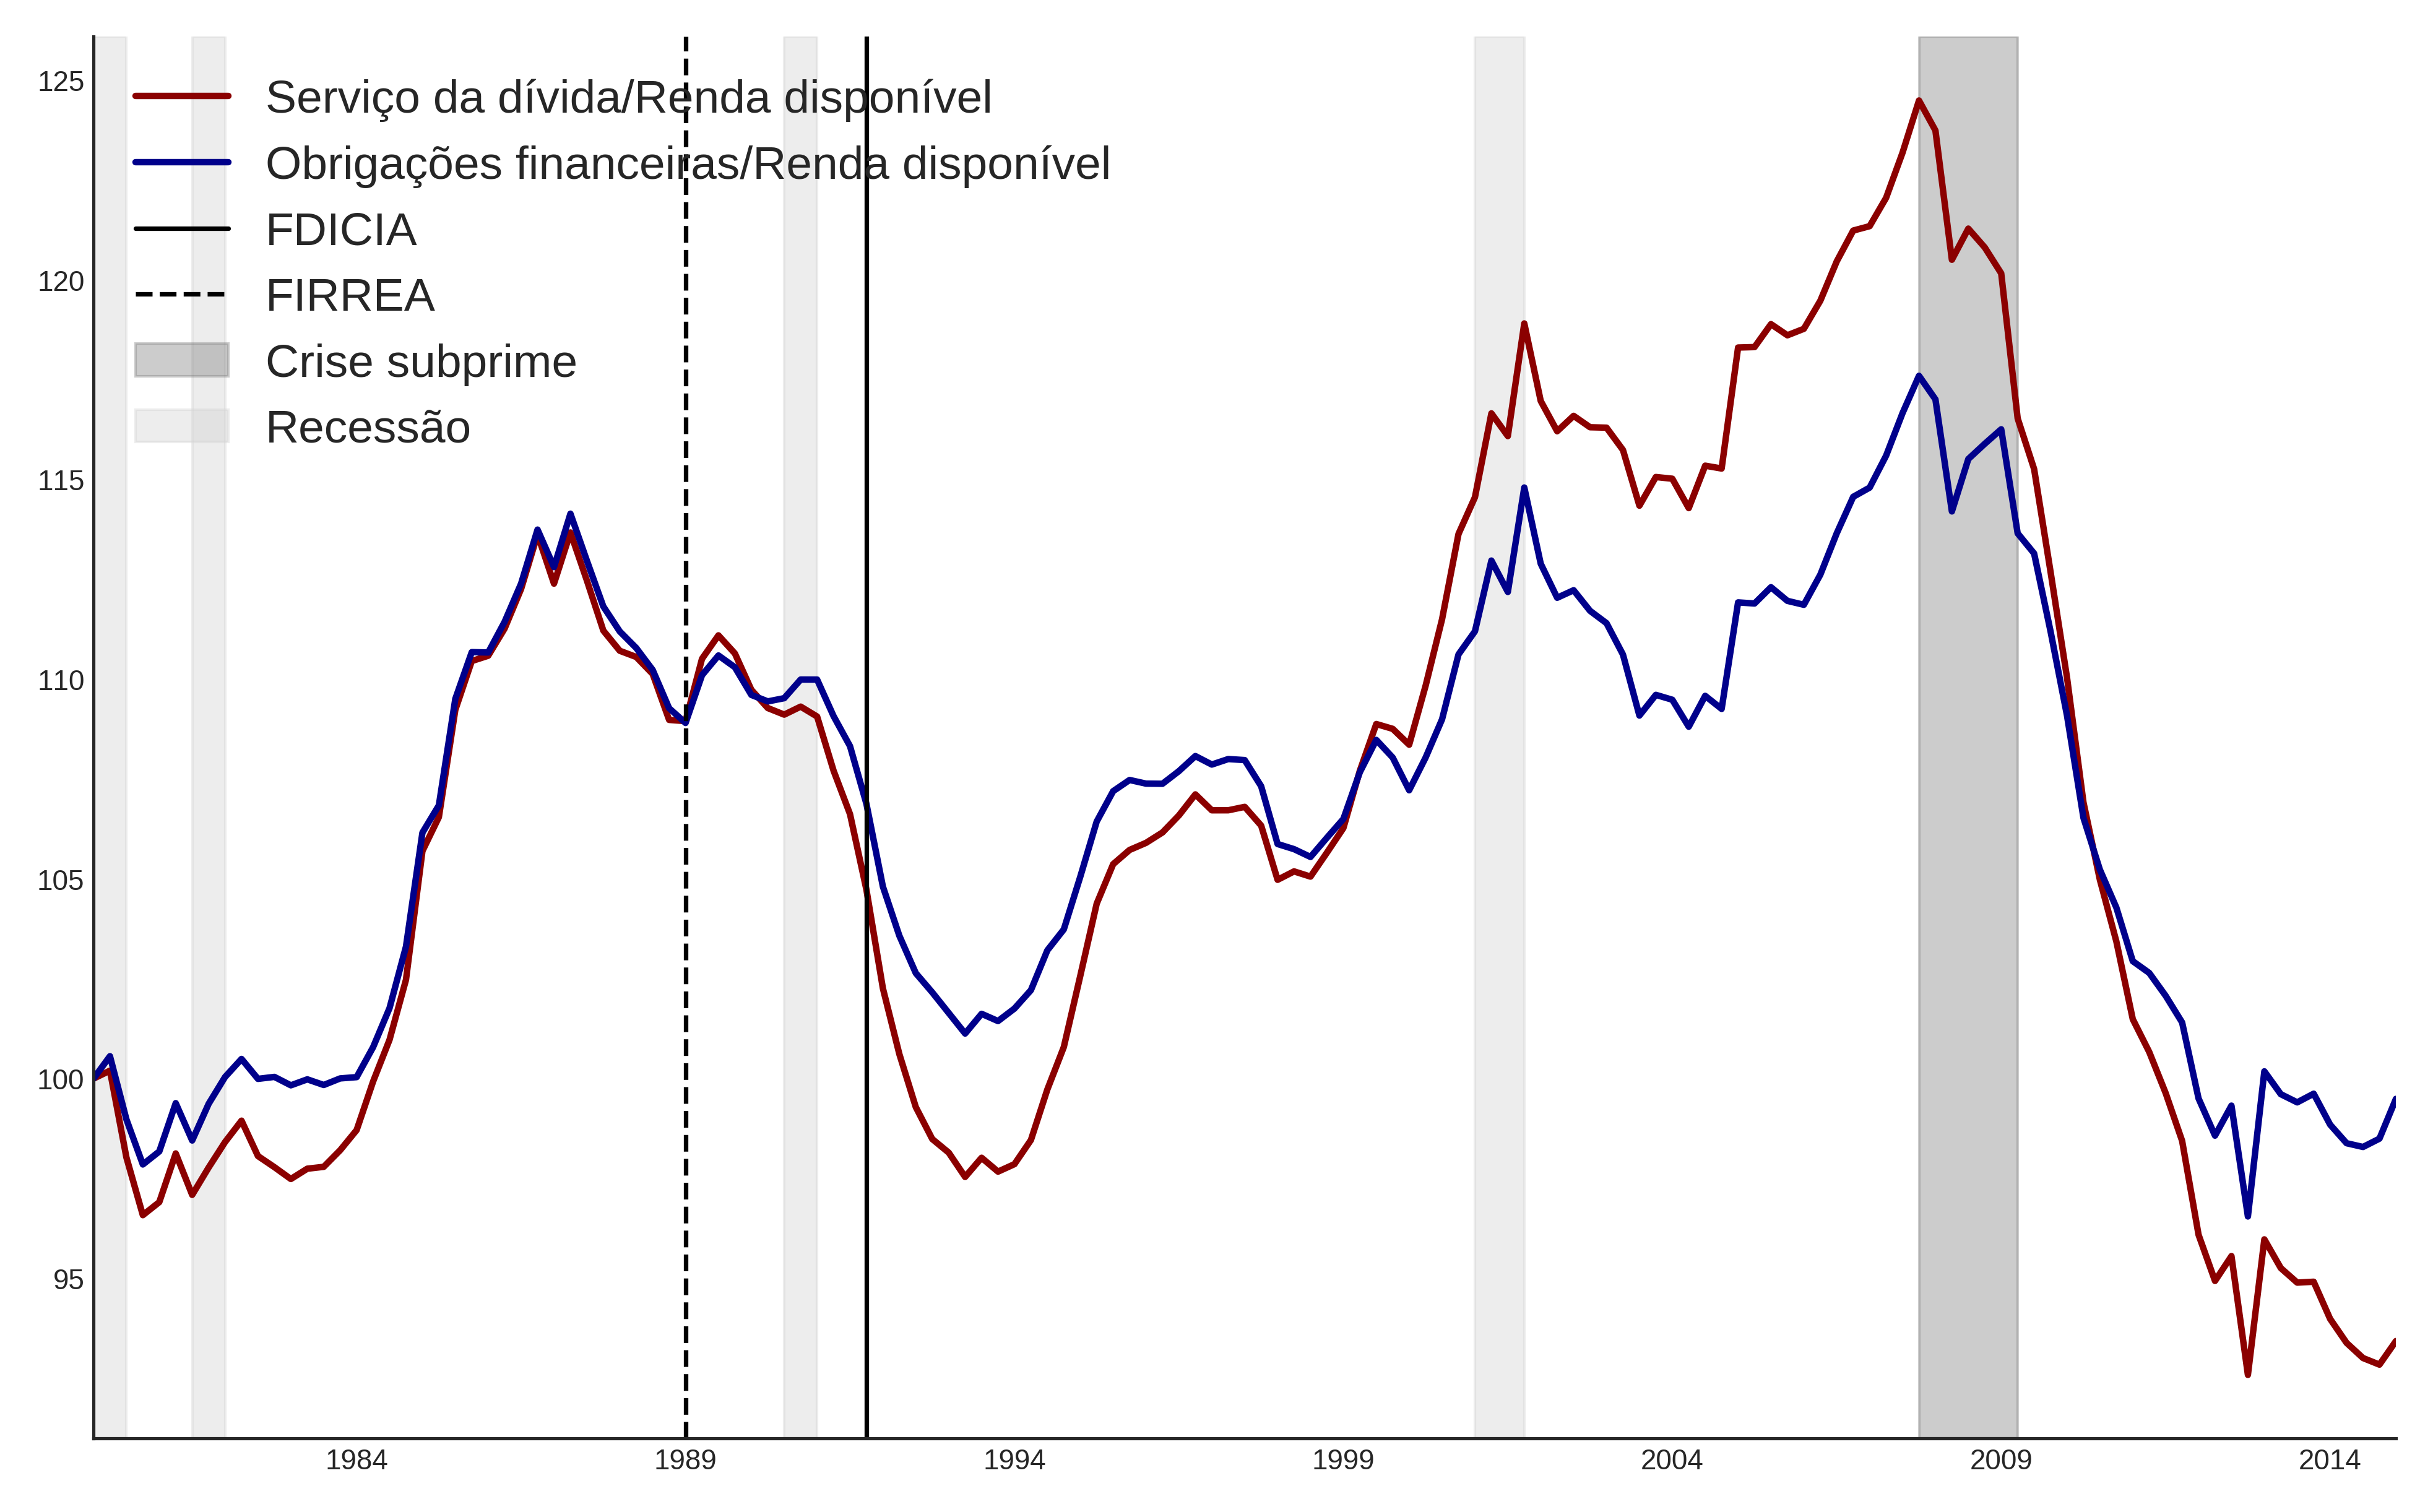
\includegraphics[width=\textwidth]{../../Dados/Fatos_Estilizados/figs/Serv_Divida.png}
%	\caption*{\textbf{Fonte:} U.S. Bureau of Economic Analisys, elaboração própria}
%\end{figure}


Existe também outra dimensão relevante que a literatura não dá a devida atenção: popularização dos imóveis primários\footnote{
	Em linhas gerais, um imóvel primário é aquele que o proprietário tem acesso regular e, no caso de possuir mais de um imóvel (secundário), é aquele que usufrui a maior parte do tempo ao longo do ano \cite{us_census_bureau_characteristics_2017}.
}.
A ampliação do acesso às residências pode ser visualizada no gráfico \ref{FigConcentracao} em que estão apresentadas as curvas de concentração\footnote{
	Em linhas gerais, curvas de concentração são elaboradas a partir da ordenação acumulada de duas variáveis distintas. O eixo horizontal do gráfico \ref{FigConcentracao} contém a proporção acumulada das famílias enquanto o eixo vertical apresenta a proporção acumulada de uma parcela da riqueza (neste caso, imóveis primários e secundários). Por fim, para construir as curvas de concentração ordena-se ambos os eixos pela riqueza total tornando-as --- diferentemente da curva de Lorenz --- não-decrescentes de modo que possam ultrapassar a linha de perfeita igualdade. Para mais detalhes, consultar \textcite[p.~197--201]{hoffmann_distribuicao_2018}.
} de 1989 a 2010 por diferentes tipos de imóveis (primários e secundários).
A partir destas curvas é possível avaliar quão concentrado é certo tipo de ativo comparando-o com a linha de perfeita igualdade\footnote{Quão mais acima e a esquerda da curva de Lorenz, menos concentrado/mais progressivo o ativo em questão está/é enquanto uma curva mais a direita e abaixo indica o oposto.
Neste caso, um ponto acima desta linha indica que o ativo em questão (neste caso, imóveis) é distribuído a favor dos estratos mais pobres da riqueza.
Além disso, a distribuição deste ativo contribuirá para a redução da desigualdade quanto mais inclinada for a curva de concentração na região dos mais pobres \cite[p.~36]{medeiros_uma_2006}.
}.
Para auxiliar a interpretação deste gráfico, toma-se o ano de 2010 como exemplo.
Neste ano, até 25\% das famílias com riqueza possuíam 21,80\% de todos os imóveis primários, enquanto as famílias até 50\%, 75\% e 90\% detinham 61,30\%, 90,10\% e 95,30\% dos imóveis respectivamente já o topo da distribuição (10\% mais ricos) possuía 97,10\% de todos os imóveis primários de modo que o restante (2,9\%) não estava sob a posse das famílias.

Dito isso, uma breve inspeção deste gráfico revela que os anos que antecederam a Grande Recessão foram caracterizados pela desconcentração dos imóveis primários, ou seja, estratos mais pobres da população passaram a deter uma parcela acumulada maior deste tipo de imóvel.
Uma vez que as residências primárias dizem respeito àquelas que são utilizadas para fins não necessariamente especulativos, verifica-se uma elevação generalizada da demanda por imóveis enquanto moradia e não enquanto ativos (ver também gráfico \ref{FigDistAtivos}).
%IMÓVEIS PRIMÁRIOS POR QUE SÃO ÚTEIS E SECUNDÁRIOS PELA ESPECULAÇÃO
O mesmo não pode ser dito sobre os imóveis secundários\footnote{
	De acordo com o \textit{Survey of Construction} \cite{us_census_bureau_characteristics_2017}, os imóveis secundários são aqueles em que: (i) os proprietários residem parte do ano apenas; (ii) está ao menos 50 milhas do imóvel primário e; (iii) não pode estar sujeito a um contrato de aluguel.
} cujo movimento de concentração/distribuição não é tão demarcado quanto no caso anterior.
Além disso, uma vez que este tipo de imóvel não é destinado ao uso regular de seu proprietário, uma maior distribuição deste ativo sugere uma ampliação da demanda por imóveis na expectativa de ganhos de capital\footnote{
	Como pontuado no corpo do texto, esta aumento da demanda por imóveis secundários \textit{pode} indicar --- mas não se restringe a --- aumento por motivos especulativos. Uma casa de férias ou para aluguel, por exemplo, são usos não-especulativos de uma residência secundária.
	De todo modo, argumenta-se que há relação entre imóveis secundários e especulação.
}\footnote{Outro elemento que chama atenção no gráfico \ref{FigConcentracao} é que as famílias mais ricas não são as principais detentoras deste tipo de riqueza uma vez que acumulam menos da metade destes imóveis ao longo do período analisado (ver eixo vertical).}.


\begin{figure}[H]
	\centering
	\caption{Curva de concentração por tipos de imóveis}
	\label{FigConcentracao}
	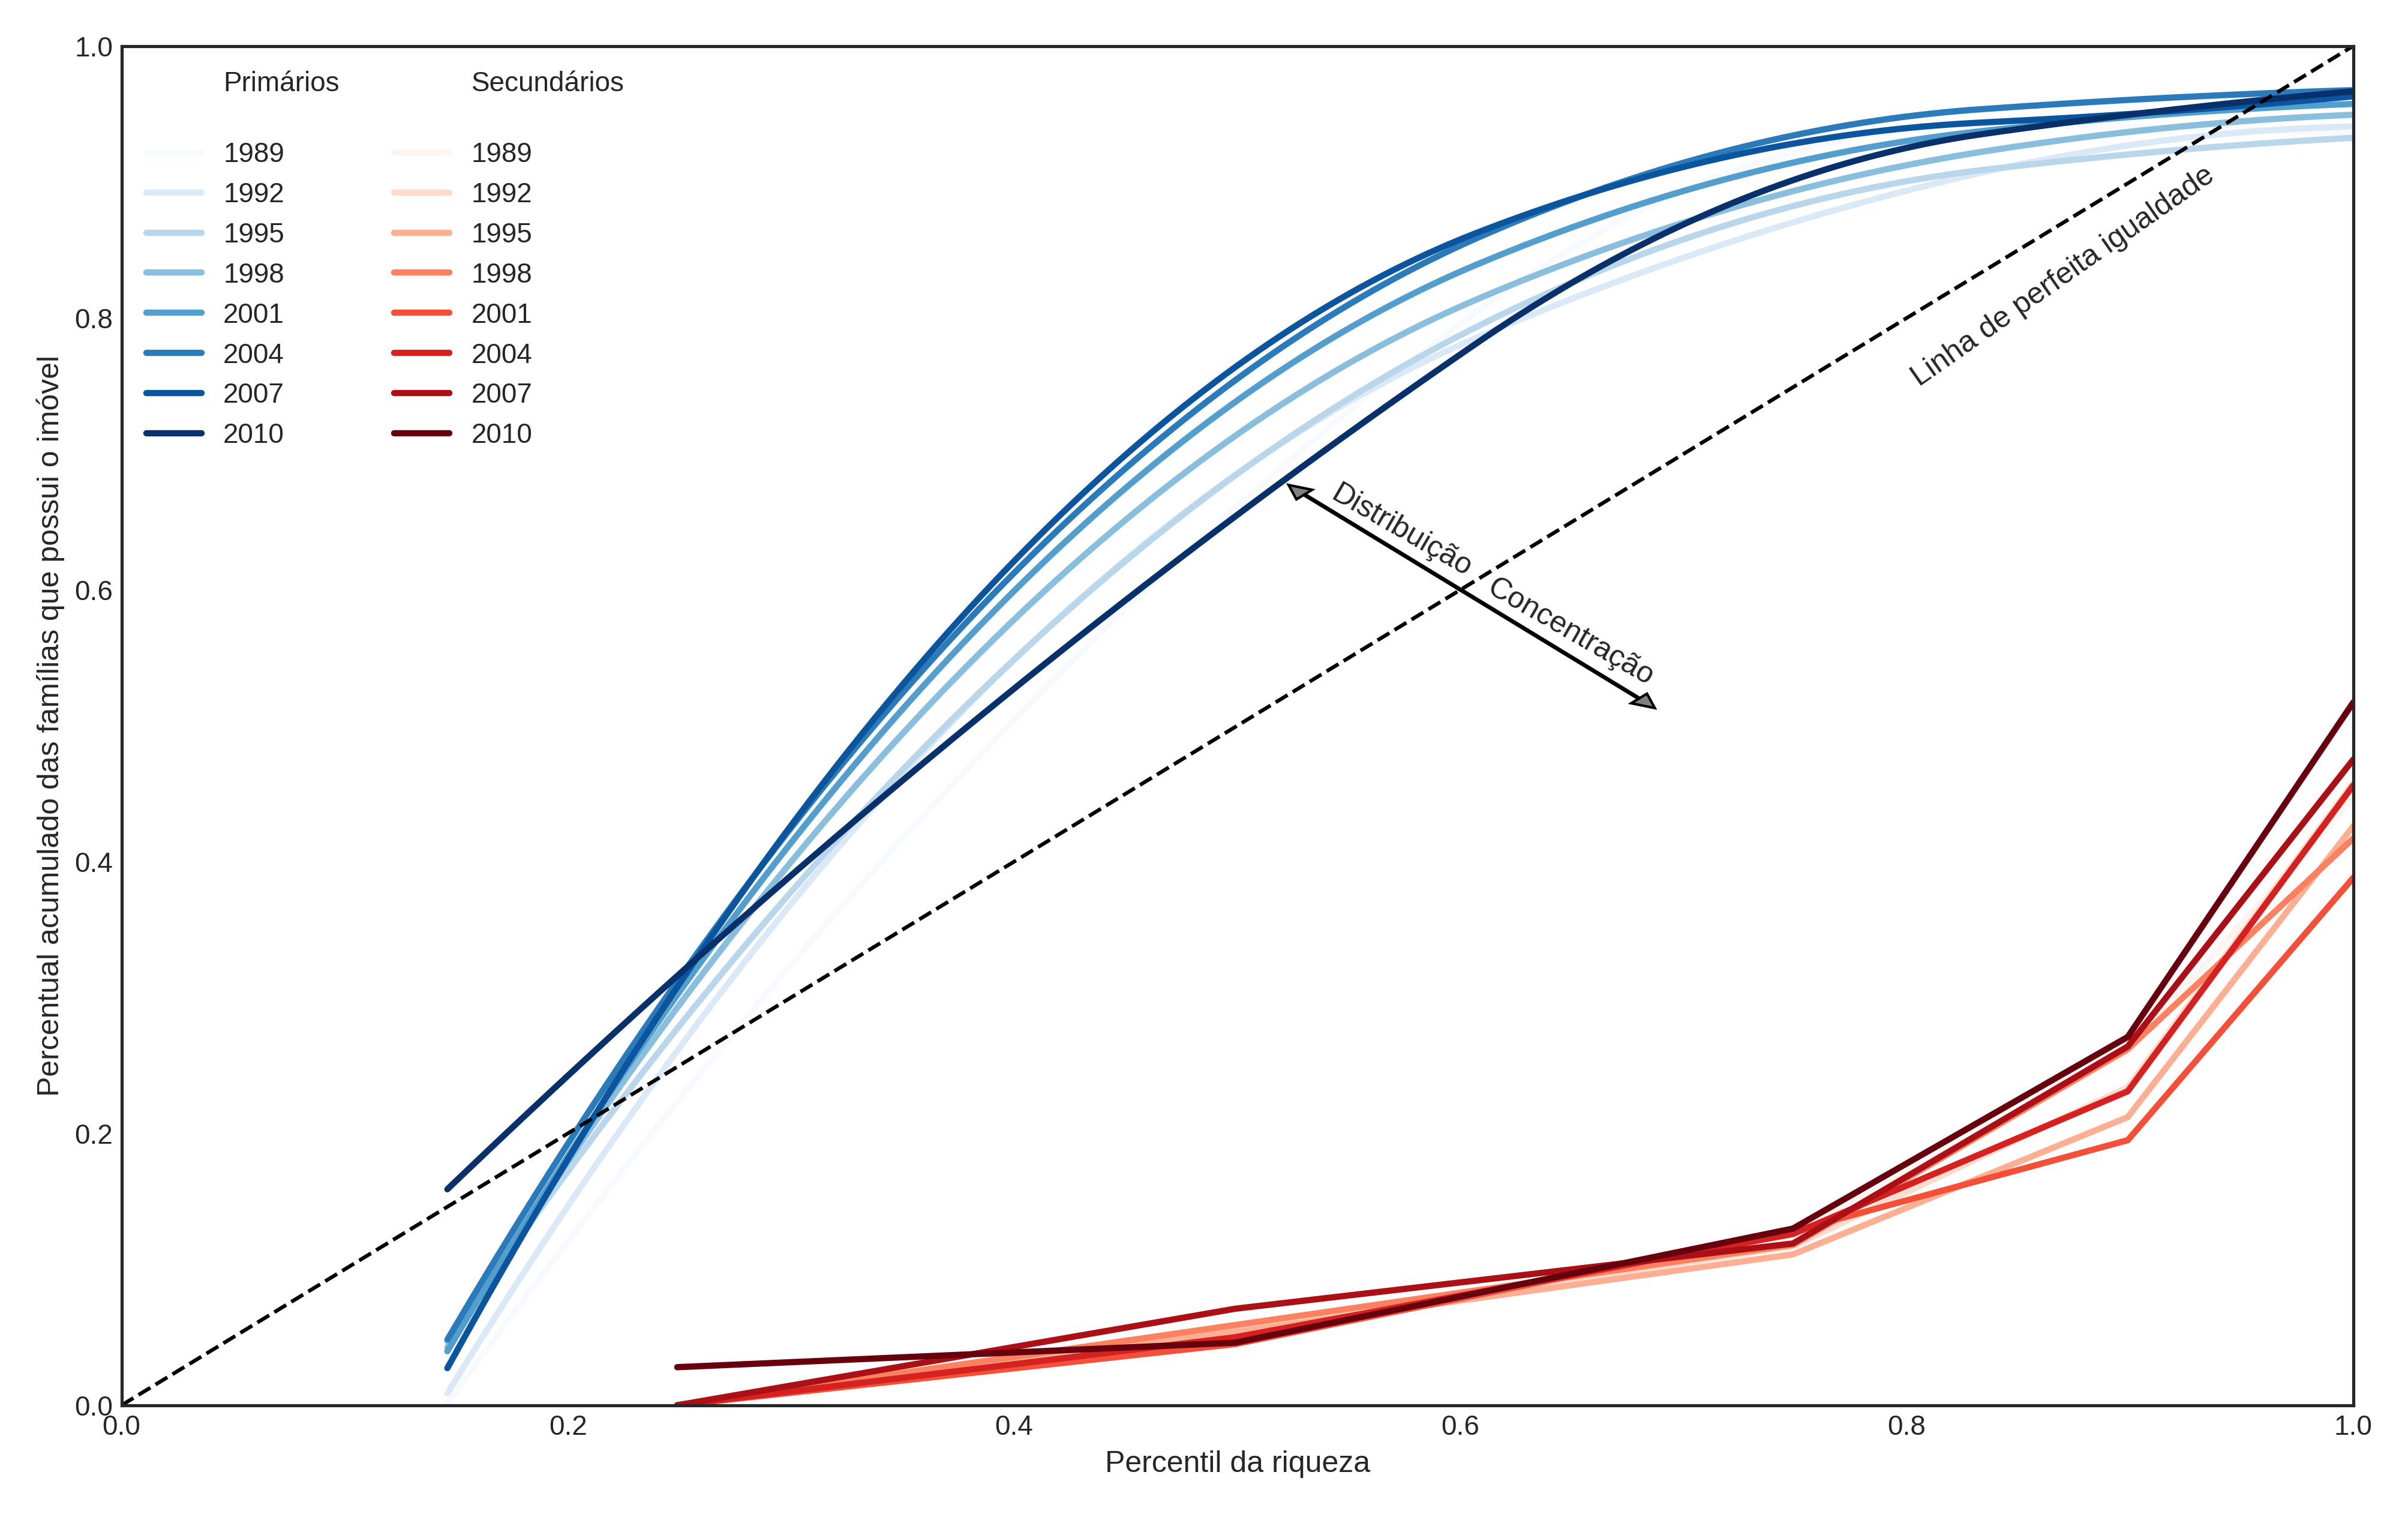
\includegraphics[width=\textwidth]{../../Dados/Fatos_Estilizados/figs/Concentracao_Imoveis.png}
	\caption*{\textbf{Fonte:} \textcite{us_census_bureau_characteristics_2017}, Elaboração própria}
\end{figure}
%Por fim, partindo da hipótese apresentada no capítulo anterior (ver equação \ref{tx_Propria}) de que o investimento residencial possui um componente de longo prazo (popularização dos imóveis, por exemplo) e outro de médio prazo (especulação), argumenta-se que a relevância do aumento generalizado da participação dos imóveis está associado  ao maior acesso ao crédito imobiliário --- sobretudo entre os estratos de renda mais baixos --- decorrente da desregulamentação financeira (ver painel inferior esquerdo dos gráficos \ref{FigDistAtivos} e \ref{FigDistPassivos}).
%Sendo assim, uma vez esgotada a bolha de ativos, os impactos são maiores que na ausência desta ``popularização residencial''.

%%%%%%%%%%%% RESUMO PARA OS CHOQUES
Em resumo, pontuou-se a relevância do investimento residencial para dinâmica macroeconômica.
Aliado a isso, outros fatos estilizados foram apresentados e que serão levados adiante nos choques do capítulo \ref{CapModelo}.
Tenho em mente a equação \ref{tx_Propria}, os choques são:
	(i) ampliação da demanda por imóveis por motivos especulativos (via aumento do coeficiente $\phi_1$);
	(ii) aumento da demanda por imóveis associada às mudanças demográficas (via aumento do coefieinte $\phi_0$);
	(iii) redução da participação dos salários na renda (por meio de alterações no \textit{wage-share})
	e;  
	(iv) maior comprometimento da renda das famílias com pagamento de juros da dívida (via aumento da taxa de juros).
Apresentados estes fatos estilizados, cabe a seção seguinte investigar como a literatura econométrica tem tratado o investimento residencial em termos macroeconômicos.

%Teixeira e a taxa própria
